% \documentclass[a4paper, 11pt]{article}
\documentclass{article}

\usepackage[dvipsnames]{xcolor}
\usepackage{ctex}
\usepackage{graphicx}
\usepackage[unicode]{hyperref}
\usepackage{cite}
\usepackage{indentfirst}
\usepackage{listings}
\usepackage{geometry}
\usepackage{amsmath}
\usepackage{tabularx}

\geometry{a4paper, left=2cm, right=2cm, top=1cm, bottom=1.5cm}

% \lstset{
%   language=C++,
%   basicstyle=\fontsize{8}{5}\ttfamily, % 设置代码字体大小为 12pt
%   breaklines=true, % 自动换行
%   numbers=left,
%   showstringspaces = false
% }

%%%%%% 设置字号 %%%%%% 
\newcommand{\chuhao}{\fontsize{nn42pt}{\baselineskip}\selectfont}
\newcommand{\xiaochuhao}{\fontsize{36pt}{\baselineskip}\selectfont}
\newcommand{\yihao}{\fontsize{28pt}{\baselineskip}\selectfont}
\newcommand{\erhao}{\fontsize{21pt}{\baselineskip}\selectfont}
\newcommand{\xiaoerhao}{\fontsize{18pt}{\baselineskip}\selectfont}
\newcommand{\sanhao}{\fontsize{15.75pt}{\baselineskip}\selectfont}
\newcommand{\sihao}{\fontsize{14pt}{\baselineskip}\selectfont}
\newcommand{\xiaosihao}{\fontsize{12pt}{\baselineskip}\selectfont}
\newcommand{\wuhao}{\fontsize{10.5pt}{\baselineskip}\selectfont}
\newcommand{\xiaowuhao}{\fontsize{9pt}{\baselineskip}\selectfont}
\newcommand{\liuhao}{\fontsize{7.875pt}{\baselineskip}\selectfont}
\newcommand{\qihao}{\fontsize{5.25pt}{\baselineskip}\selectfont}

% %%%% 设置 section 属性 %%%%
% \makeatletter
% \renewcommand\section{\@startsection{section}{1}{\z@}%
% {-1.5ex \@plus -.5ex \@minus -.2ex}%
% {.5ex \@plus .1ex}%
% {\normalfont\sihao\CJKfamily{hei}}}
% \makeatother

 %%%% 设置 subsection 属性 %%%%
% \makeatletter
% \renewcommand\subsection{\@startsection{subsection}{1}{\z@}%
% % {-1.25ex \@plus -.5ex \@minus -.2ex}%
% % {-1ex \@plus -.5ex \@minus -.2ex}%
% {-1ex \@plus -.3ex \@minus -.1ex}%
% {.4ex \@plus .1ex}%
% {\normalfont\xiaosihao\CJKfamily{hei}}}
% \makeatother

% %%%% 设置 subsubsection 属性 %%%%
% \makeatletter
% \renewcommand\subsubsection{\@startsection{subsubsection}{1}{\z@}%
% {-1ex \@plus -.5ex \@minus -.2ex}%
% {.3ex \@plus .1ex}%
% {\normalfont\xiaosihao\CJKfamily{hei}}}
% \makeatother

%%%% 段落首行缩进两个字 %%%%
\makeatletter
\let\@afterindentfalse\@afterindenttrue
\@afterindenttrue
\makeatother
% \setlength{\parindent}{2em}  %中文缩进两个汉字位

%%%% 下面的命令重定义页面边距,使其符合中文刊物习惯 %%%%
% \addtolength{\topmargin}{-54pt}
% \setlength{\oddsidemargin}{0.63cm}  % 3.17cm - 1 inch
% \setlength{\evensidemargin}{\oddsidemargin}
% \setlength{\textwidth}{14.66cm}
% \setlength{\textheight}{24.00cm}    % 24.62

%%%% 下面的命令设置行间距与段落间距 %%%%
\linespread{1.0}
% \setlength{\parskip}{1ex}
\setlength{\parskip}{0.5\baselineskip}

% 在导言区进行样式设置
\lstset{
    language=C++, % 设置语言
 	basicstyle=\ttfamily, % 设置字体族
 	breaklines=true, % 自动换行
 	keywordstyle=\bfseries\color{NavyBlue}, % 设置关键字为粗体,颜色为 NavyBlue
 	morekeywords={PressureSensor, Button, Oled}, % 设置更多的关键字,用逗号分隔
 	emph={self}, % 指定强调词,如果有多个,用逗号隔开
    emphstyle=\bfseries\color{Rhodamine}, % 强调词样式设置
    commentstyle=\itshape\color{black!50!white}, % 设置注释样式,斜体,浅灰色
    stringstyle=\bfseries\color{PineGreen!90!black}, % 设置字符串样式
    columns=flexible,
    numbers=left, % 显示行号在左边
    numbersep=2em, % 设置行号的具体位置
    numberstyle=\footnotesize, % 缩小行号
    % frame=single, % 边框
	tabsize = 4,  %行缩进
    framesep=1em % 设置代码与边框的距离
}

%%%% 正文开始 %%%%
\begin{document}	
		%%%% 定理类环境的定义 %%%%
\newtheorem{example}{例}             % 整体编号
\newtheorem{algorithm}{算法}
\newtheorem{theorem}{定理}[section]  % 按 section 编号
\newtheorem{definition}{定义}
\newtheorem{axiom}{公理}
\newtheorem{property}{性质}
\newtheorem{proposition}{命题}
\newtheorem{lemma}{引理}
\newtheorem{corollary}{推论}
\newtheorem{remark}{注解}
\newtheorem{condition}{条件}
\newtheorem{conclusion}{结论}
\newtheorem{assumption}{假设}

		%%%% 重定义 %%%%
\renewcommand{\contentsname}{目录}  % 将Contents改为目录
\renewcommand{\abstractname}{摘要}  % 将Abstract改为摘要
\renewcommand{\refname}{参考文献}   % 将References改为参考文献
\renewcommand{\indexname}{索引}
\renewcommand{\figurename}{图}
\renewcommand{\tablename}{表}
\renewcommand{\appendixname}{附录}
\renewcommand{\algorithm}{算法}	

		%%% 定义标题格式,包括title,author,affiliation,email等 %%%%
\title{智能仓储系统的开发研究}
% \author{XXX\footnote{电子邮件: XXXXXXXXXXXX@zjut.edu.cn 学号: XXXXXXXXXXXX}\\[2ex]
% \xiaosihao 浙江工业大学\\[2ex]}
\author{\xiaosihao 先进计算与机器人研究所}
%\date{}
		
		%%%% 以下部分是正文 %%%%  
\maketitle
		
\tableofcontents
\newpage

\section{第一章: 压力测量模块}

\begin{figure}[h]
	\centering
	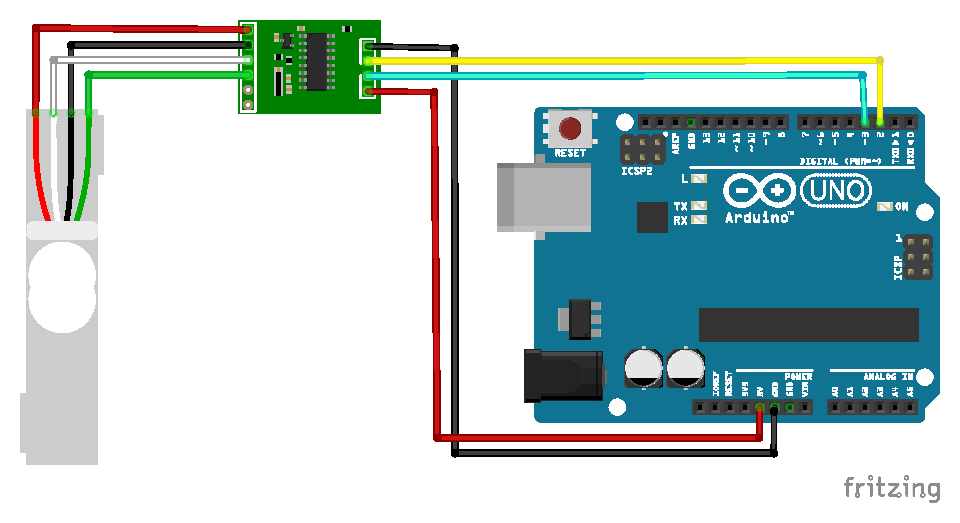
\includegraphics[width=\linewidth]{../1_Chapter1_RAW/Picture/PressureSensor.pdf}
	\caption{压力测量模块流程}
	\label{fig:压力测量模块流程图}
	\hfill
\end{figure}
		
	压力测量模块的连线:
\begin{itemize}
	\item 称重传感器的红线代表电源正极, 连接HX711 模块的 E+ 引脚
	\item 称重传感器的黑线代表电源负极, 连接HX711 模块的 E- \hspace{0.5em}引脚
	\item 称重传感器的白线代表信号输出, 连接HX711 模块的 A- \hspace{0.5em}引脚
	\item 称重传感器的绿线位保留线, 连接HX711 模块的 A+ 引脚		
	\item HX711 模块的GND引脚连接 arduino 的GND引脚
	\item HX711 模块的VCC引脚连接 arduino 的5V引脚
	\item HX711 模块的DT\hspace{0.5em} 引脚连接arduino的任意数字引脚pin\_DT(下文为数字引脚3), 在构造函数里会将Arduino中的该引脚
	设置为输入模式, 用于接收HX711传来的数字信号。
	\item HX711 模块的SCK引脚连接 arduino 的任意数字引脚pin\_SCK(下文为数字引脚2), 在构造函数里会将Arduino中的该引脚设置为输出模式,
	用于发送脉冲, 然后HX711会按数位输出数据到pin\_DT。
\end{itemize}

初始秤的计算步骤
\begin{itemize}
  \item 1. 获得空秤时的AD值;
  \item 2. 获得物体称重结果;
\end{itemize}

\subsection{获得空秤时的AD\_Surface值}
Surface类是用于读写arduino上地址0到3储存的unsigned long AD\_Surface, AD\_Surface是指没放待测物体时HX711的读数,
在待测物体称重时都要减去这个关键值。有必要在arduino上存下这个值, 并且断电重启后还在。所以创建了这个类来表示相关变量和函数:

\begin{lstlisting}
class Surface{
union coeffience {
  unsigned long value_out;
  byte value_in[4];
};

private:
  int pin_SCK, pin_DT, range; 
  bool flag;
  unsigned long AD_Surface;

  unsigned long HX711_Read();

public:
  Surface();
  void setpin_SCKDT(int p1, int p2);
  unsigned long Get_Surface();
};
\end{lstlisting}

因为arduino上一个地址只能存一个字节, AD\_Surface是四个字节表示的long型数据, 故需要4个地址来储存。而为了方便读写, 这里先创建一个共用体coeffience,
有了共用体coeffience后, 当某coeffience型变量a的变量类型value\_out和value\_in中的任意一个赋值后, 可以直接转化成另一个类型:
\begin{lstlisting}
union coeffience {
    unsigned long value_out;
    byte value_in[4];
};
\end{lstlisting}

这个共用体可以表示为unsigned long和byte数组两种形式, 在Get\_Surface函数会用这个共用体来读写aurdino硬盘上储存的AD\_Surface。

私有成员: \\
\romannumeral1.	Arduino上连的数字引脚pin\_SCK, pin\_DT;\\
\romannumeral2. flag是为了区分是否要计算AD\_Surface值, 不计算在默认构造函数里设为0, 反之在setpin\_SCKDT设为1;\\
\romannumeral3. AD\_Surface是指没放待测物体时HX711的读数。\\
\romannumeral4. HX711\_Read()是读取AD值, 将在1.4, 1.5小节详细介绍。\\

下面是公用成员函数部分。默认构造函数做了两件事情, 一件是从arduino内置硬盘读取之前存的AD\_Surface, 用一个for循环访问地址0到3, 并将每次读到的值保存在变量memory中, 再赋给AD\_Surface作为初值,
如果没有存过, 则读到的值为0;还有一件是flag初始化为0, 表示准备利用读取的AD\_Surface来进行接下来的称重计算。
\begin{lstlisting}
Surface::Surface(){
  coeffience memory;
  for (int i=0; i<4; ++i)
    memory.value_in[i]=EEPROM.read(i);
  AD_Surface = memory.value_out;
  flag=0;
};  
\end{lstlisting}

setpin\_SCKDT(int, int)用于设置SCK, DT连接的引脚, 然后就是设置引脚的输出模式。设置Arduino上数字信号引脚pin\_SCK、pin\_DT
分别为输出模式和输入模式, 分别用于将电压信号输出给HX711上SCK端和接受HX711中DT端传导来的数字信号。如果在主程序setup里用到了这个函数, 说明是打算重新计算AD\_Surface的, 
所以在这个函数里, flag设为1; 如果在setup里没有设置Surface的引脚, 则是打算只利用板上已存的信息进行之后的称重计算。\\
\begin{lstlisting}
void Surface::setpin_SCKDT(int p1, int p2) {
  pin_SCK = p1;
  pin_DT = p2;
  pinMode(pin_SCK, OUTPUT);	
  pinMode(pin_DT, INPUT);	
  flag=1;
}
\end{lstlisting}

因为核心函数Get\_Surface()要调用到HX711\_Read()函数(这个函数会在本章最后两节介绍)。
在Surface类初始化的时候, flag为0。Get\_Surface()通过flag是否为1来判断是否要重新读一次当前AD值。
如果flag为1就进行arduino板的写入操作, 反之就仅仅读arduino板。最终返回的是AD\_Surface。
\begin{lstlisting}
unsigned long Surface::Get_Surface(){
  if (flag) {
    unsigned long AD_Sum=0, AD_Read=0;
    for (int i=0; i<10; ++i){
      AD_Read = HX711_Read();
      Serial.println(AD_Read);
      AD_Sum+=AD_Read;
    } 
    AD_Surface = AD_Sum/10;

    coeffience AD_Surface_out;
    AD_Surface_out.value_out = AD_Surface;

    for(int i=0; i<4; i++)   
      if (!(EEPROM.read(i)==AD_Surface_out.value_in[i])) {
        Serial.println("OVERWRITE");
        for (int i=0; i<4; i++) 
          EEPROM.write(i, AD_Surface_out.value_in[i]);
        break;
      }
  flag = 0;
  }
  Serial.println(AD_Surface);
  return AD_Surface;
};
\end{lstlisting}

在flag为1时, 主要做了两件事情, \\
\noindent 1. 读取十次没有放置待测物体时压力传感器的AD值, 取平均后保存在AD\_Surface。\\
\noindent 2. 把AD\_Surface与arduino之前存的AD\_Surface做对比, 如果发生改变, 则在相同位置全部覆盖写入, 这样断电重启后也能直接读到。

首先是取平均值存入AD\_Surface, 即更新Surface类中的变量AD\_Surface:
\begin{lstlisting}
void Surface::Get_Surface(){
  unsigned long AD_Sum=0;
  for (int i=0; i<10; ++i) 
    AD_Sum+=ps.HX711_Read();
  AD_Surface = AD_Sum/10;
\end{lstlisting}

下面代码将AD\_Surface存到了共用体AD\_Surface\_out中。
\begin{lstlisting}
coeffience AD_Surface_out;
AD_Surface_out.value_out = AD_Surface;
\end{lstlisting}

最多循环四次比较所有地址上存储的数, 发现不同就从第一个位置开始逐位写入arduino。
\begin{lstlisting}
for(int i=0; i<4; i++)
  if (!(EEPROM.read(i)==AD_Surface_out.value_in[i])) {
    for (int i=0; i<4; i++) 
      EEPROM.write(i, AD_Surface_out.value_in[i]);
    break;
  }  
\end{lstlisting}

\subsubsection{Surface.ino}
\begin{lstlisting}
#include "Surface.h"
Surface s;
void setup() {
  Serial.begin(9600);
  s.setpin_SCKDT(4, 5);
  s.Get_Surface();
}

void loop() {}
\end{lstlisting}

\subsection{获得物体称重结果}
下面将进行理论上准确的称重步骤, 我们将先得到称重结果, 并在图像上和真实重量对比。具体称重理论放在set\_range函数部分介绍。
称重的核心函数是Output\_Weight(),得到的是以克为单位的真实质量RealWeight, HX711\_Read()读取HX711AD模块上储存的数字信号函数, 
返回代表数字信号的AD值,计算原理放在1.4节和1.5节介绍。这里传进来的参数是AD\_Surface, 在本章第一节里介绍过。
\begin{lstlisting}
void PressureSensor::Output_Weight(unsigned long ADS) {
  unsigned long difference = HX711_Read() - ADS;
  return (long)(difference/GapValue);;
};
\end{lstlisting}
称重分为三步:\\
\noindent 第一步: 用HX711\_Read()读取放入待测物体后的AD值, \\
\noindent 第二步: 减去没放待测物体时的AD值ADS, 储存在中间变量difference中;\\
\noindent 第三步: 将第一步得到的结果除以刚刚提到的转化系数GapValue, 返回的计算结果就是不准的称重质量;\\

介绍PressureSensor类的成员构成, 
\begin{lstlisting}
class PressureSensor {

private:
  int pin_SCK, pin_DT, range;
  float GapValue;

public:
  PressureSensor();
  void setpin_SCKDT(int p1, int p2);
  void set_range(int r);
  unsigned long Output_Weight(unsigned long ADS);
  unsigned long HX711_Read();
};
\end{lstlisting}

私有变量: \\
\romannumeral1.	Arduino上连的数字引脚pin\_SCK, pin\_DT, 压力传感器的量程range;\\
\romannumeral2. HX711AD模块读到的数转化成质量(以克为单位)时用到的系数GapValue;\\

公共成员函数: \\
默认构造函数:
\begin{lstlisting}
PressureSensor::PressureSensor(){};
\end{lstlisting}

setpin\_SCKDT(int, int)用于设置SCK, DT连接的引脚, 然后就是设置引脚的输出模式。设置Arduino上数字信号引脚pin\_SCK、pin\_DT
分别为输出模式和输入模式, 分别用于将电压信号输出给HX711上SCK端和接受HX711中DT端传导来的数字信号。;\\
\begin{lstlisting}
void PressureSensor::setpin_SCKDT(int p1, int p2) {
  pin_SCK = p1;
  pin_DT = p2;
  pinMode(pin_SCK, OUTPUT);	
  pinMode(pin_DT, INPUT);	
}
\end{lstlisting}

set\_range(int)传入当前传感器的量程, 并计算得到一个转化系数GapValue。\\
\noindent 注: 因为通过压力传感器读到的信号不是真实的质量, 
我们需要一个系数把这个转换成以克(g)为单位的数字。假设被测物体的重量x(kg), 而所能从HX711AD模块得到的只有AD值y, 
因此这里已知压力传感器的最大量程range(kg), AD值最大值为(由1.5中式(4)可知),

\begin{equation}
	AD_{max} = 0.128\times(2^{24}-1)
\end{equation}

可以得到其中的转换关系:

\begin{equation}
	x = \frac{y}{0.128\times(2^{24}-1)}\times range\times 10^3
\end{equation}

这里:
\begin{equation}
	GapValue = \frac{128\times(2^{24}-1)\times 10^{-6}}{range}
\end{equation}

在最大量程rangekg已知的情况下, GapValue便成为一个常量(16.777216 为2的24次方除以1000000), 因此在程序中给定量程后, 便可以得到GapValue对应的值。

\begin{lstlisting}
void PressureSensor::set_range(int range) {
  GapValue = 128 * 16.777215 / range;
};
\end{lstlisting}

\subsubsection{PressureSensor.ino}
连接Arduino板后, 编译上传该主程序及相关头文件即可实现压力测量模块的全部功能。

\begin{lstlisting}
#include "PressureSensor.h"
#include "Surface.h"

PressureSensor YL;
Surface YL_Surface;

void setup() {
  Serial.begin(9600);
  YL.setpin_SCKDT(4, 5);
  YL.set_range(20);
  YL_Surface.setpin_SCKDT(4, 5);
}

void loop() {
  unsigned long RealWeight = YL.Output_Weight(YL_Surface.Get_Surface());
  Serial.println(RealWeight);
  delay(1000);
}
\end{lstlisting}

\subsection{称重结果可视化}
我们猜测目前的秤不准的读数x和准确的质量y之间是一个线性关系, 可以用$y=kx+b$表示。为了大致看看数据, 在PressureSensor类的基础上添加了数组x[13], 与x数组
长度保持一致的整数n, 和获得这个数组的函数Get\_x\_array, 以及计算线性系数的函数Get\_kb。为了与PressureSensor类区分开来, 新建了Calibrate类。

这一节核心就是两步: 获得x数组; 计算kb。

\begin{lstlisting}
class Calibrate {
union coeffience {
  unsigned long value_out;
  byte value_in[4];
};

private:
  int pin_SCK, pin_DT, range; 
  float GapValue;
  unsigned long k, b;
  unsigned long x[13];
  int n;

public:
  Calibrate();

  void Get_x_array(unsigned long ADS);
  void Get_kb();
  void setpin_SCKDT(int p1, int p2);
  void set_range(int r);
  unsigned long Output_Weight(unsigned long ADS);
  unsigned long HX711_Read();
};
\end{lstlisting}

除了Get\_x\_array和Get\_kb, 其他函数与之前所提到的一样。
首先是Get\_x\_array函数。n为13, 是因为预先设置好的测试数组长度为13:
\begin{lstlisting}
void Calibrate::Get_x_array(unsigned long ADS){
  n=13;
  Serial.println("CARLIBRATING, NOW");
  delay(5000);
  Serial.println("START");
  delay(2000);
  for (int i=0; i<n; i++) {
    Serial.print("x");
    Serial.print(i+1);
    Serial.print(": ");
    delay(5000);
    x[i] = Output_Weight(ADS);
    Serial.print(x[i]);
    Serial.println("");
  }
  delay(4000); 
};
\end{lstlisting}

根据提示信息依次放置13次砝码, 每次串口打印出“x:”就是提示在5秒内放入砝码, 然后调用一次Output\_Weight(),
依次将返回值更新到x数组, 在串口打印当前存储的x[i]:
\begin{lstlisting}
  for (int i=0; i<n; i++) {
    Serial.print("x");
    Serial.print(i+1);
    Serial.print(":");
    delay(5000);
    x[i] = Output_Weight(ADS);
    Serial.print(x[i]);
    Serial.println("");
  }
\end{lstlisting}

接下来是计算拟合系数:
\begin{lstlisting}
void Calibrate::Get_kb(){
  unsigned long y[n] = {500, 1000, 1580, 2160, 2740, 3320, 13320, 12820, 12320, 11740, 11160, 10580, 10000}, sum_x = 0, sum_y = 0;
  for (unsigned long& yi:y) 
      sum_y+=yi;
  for (unsigned long& x_i:x) 
      sum_x+=x_i;
  unsigned long mean_x = sum_x/n, mean_y = sum_y/n;
  unsigned long k1=0, k2=0;
  for (int i=0; i<n; ++i) {
    k1+=x[i]*y[i];
    k2+=x[i]*x[i];
  }
  k = (k1-n*mean_x*mean_y)/(k2-n*mean_x*mean_x);
  b = mean_y - mean_x * k;

  Serial.print("k:");
  Serial.println(k);
  Serial.print("b:");
  Serial.println(b);
};

\end{lstlisting}

计算kb中, 初始化预设的准确读数, 并为砝码读数求和做准备。
其中y储存的是放入n次砝码后的标准读数(这里n=13), sum\_x是表示standards数组的求和, sum\_y是表示y数组的求和, mean\_y是数组y的平均值, 
然后对y数组, standards数组求和求平均, 分别保存在mean\_x和mean\_y, 计算拟合系数的中间变量k1, k2初始为0:

\begin{lstlisting}
unsigned long y[n] = {500, 1000, 1580, 2160, 2740, 3320, 13320, 12820, 12320, 11740, 11160, 10580, 10000}, sum_x = 0, sum_y = 0;
for (unsigned long& yi:y) 
    sum_y+=yi;
for (unsigned long& x_i:x) 
    sum_x+=x_i;
unsigned long mean_x = sum_x/n, mean_y = sum_y/n;
unsigned long k1=0, k2=0;  
\end{lstlisting}

用中学最小二乘法公式计算斜率, 其中$k_1 = \sum xy$, $k_2 = \sum x^2$
\begin{equation}
	k = \frac{\sum xy - n\overline{x}\overline{y}}{\sum x^2 - n \overline{x}^2}
\end{equation}

\begin{equation}
	b = \overline{y}- k \overline{x}
\end{equation}

\begin{lstlisting}
  for (int i=0; i<n; ++i) {
    k1+=x[i]*y[i];
    k2+=x[i]*x[i];
  }
  k = (k1-n*mean_x*mean_y)/(k2-n*mean_x*mean_x);
  b = mean_y - mean_x * k;
\end{lstlisting}
拟合的结果更新在k, b中。

实际测量中, 如图2所示
\begin{itemize}
  \item x数组为[467, 934, 1476, 2020, 2562, 3104, 11722, 11016, 10664, 10287, 9829, 9216, 8886]
  \item y数组为[500, 1000, 1580, 2160, 2740, 3320, 13320, 12820, 12320, 11740, 11160, 10580, 10000]
  \item k=1, b=851
\end{itemize}
\begin{figure}[h]
	\centering
	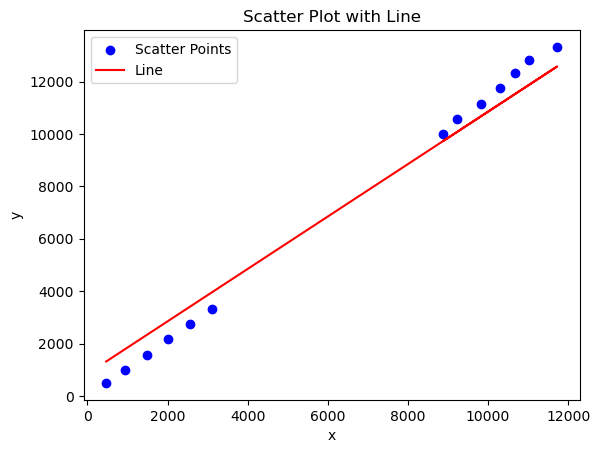
\includegraphics[width=0.5\linewidth]{../1_Chapter1_RAW/Picture/draw.png}
	\caption{称重结果}
	\label{fig:称重结果}
	\hfill
\end{figure}

\subsubsection{Draw.ino}
\begin{lstlisting}
#include "Surface.h"
#include "Calibrate.h"

Surface YL_Surface;
Calibrate YL_Calibrated;

bool flag=1;

void setup() {
  Serial.begin(9600);
  YL_Calibrated.setpin_SCKDT(4, 5);
  YL_Calibrated.set_range(20);
  YL_Surface.setpin_SCKDT(4, 5);
}

void loop() {
  if (flag) {
    YL_Calibrated.Get_x_array(YL_Surface.Get_Surface());
    YL_Calibrated.Get_kb();
    flag=0;
  }
}
\end{lstlisting}

\subsection{常用函数HX711\_Read(part 1)}
HX711\_Read()是用来得到HX711AD模块读到的电压信号。HX711AD模块在连接压力传感器后, 可以将压力传感器所传出的电压信号(一种模拟信号)
转换成AD值(一种数字信号)。其内部实现是通过建立一个电压值(模拟信号)与24位的二进制数(数字信号)的对应关系表。 
在前面我们指定了与HX711\_SCK和HX711\_DT相连的引脚pin\_SCK和pin\_DT, 在HX711\_Read()中, pin\_SCK主要是输出脉冲到
HX711\_SCK, pin\_DT主要是输入HX711\_DT传来的数字信号。其中前24次脉冲分别使得pin\_DT读到二进制数的所有数位上的数。在此之后,
可以选择再进行第25次或第26次或第27次脉冲, 其作用用于确认压力传感器输入到HX711AD模块的输入通道种类(分为AB两种)以及增益倍数, 
具体规律如下表。

\begin{tabular}{|c|c|c|}
\hline
SCK脉冲数&输入通道&增益\\
\hline
25&A&128\\
\hline
26&B&32\\
\hline
27&A&64\\
\hline
\end{tabular}

硬件连接上也有对应的要求, 当压力传感器的输出信号线选择A通道(即白线和绿线连接HX711AD模块的A-和A+引脚时), 如果只发送25次脉冲并成功发送,
压力传感器输出的信号会得到128倍增益, 此时HX711AD模块接收到的模拟信号为:$\frac{x}{A} \times VAVDD\times 128\times 1 mv/V $。
HX711AD模块的引脚E+上的输出电压就是VAVDD, E-上的输出电压为VGND(因为接地了, VGND值为0)。在每次测量压力时, 压力传感器收到
HX711AD模块发送的VAVDD作为激励电压后, 会返回$\frac{x}{A} \times VAVDD \times$ 灵敏度 (这里压力传感器的灵敏度为1mv/V, 
具体值的大小可能存在误差, 但下文用此数值代替)。考虑到信号增益倍数128以及VAVDD与HX711AD模块的最大储存值$2^{24}-1$, 可以得到AD最大值

\begin{equation}
	\begin{aligned}
		AD_{max} &= \frac{x}{range} \times VAVDD \times 0.001 \times 128 \times \frac{2^{24}-1}{VAVDD} \\
	     		 &= 0.128 \times (2^{24}-1)\\
	\end{aligned}
\end{equation}

\begin{lstlisting}
	unsigned long PressureSensor::HX711_Read() {
  	unsigned long AD_value=0;
	digitalWrite(pin_DT, HIGH);
	delayMicroseconds(1);
	digitalWrite(pin_SCK, LOW);
	delayMicroseconds(1);
	while(digitalRead(pin_DT)); 
	
	for(unsigned char i=0;i<24;++i) {
		digitalWrite(pin_SCK, HIGH); 
		delayMicroseconds(1);
		AD_value <<= 1; 
		digitalWrite(pin_SCK, LOW); 
		delayMicroseconds(1);
		if(digitalRead(pin_DT)) ++AD_value; 
	}
	
	digitalWrite(pin_SCK, HIGH); 
	delayMicroseconds(1);
	digitalWrite(pin_SCK, LOW); 
	delayMicroseconds(1);

	return AD_value;
};
\end{lstlisting}

HX711的读取是整个压力测量模块用到的最多的函数。可以分成三大部分来看:\\
\noindent 第一步: 准备开始读取信号。这一步也要做四件事情:

\noindent \uppercase\expandafter{\romannumeral1}. 局部变量AD\_value赋值为0。这里选用unsigned long类型是因为, 
设压力传感器的量程为range, 量程对应的AD值即为AD值的最大值, 经过计算可以得到,$AD_{max} = 128 \times 0.001 \times (2^{24}-1) = 0.128 \times (2^{24}-1)$ 。
由于AD值理论上只有正数, 并且在Arduino 中,unsigned long型的变量可以存储的值的范围为$0\sim2^{32}-1$,
因此这里选择用unsigned long型变量进行存储;

\begin{lstlisting}
unsigned long AD_value=0;
\end{lstlisting}	

\noindent \uppercase\expandafter{\romannumeral2}. pin\_DT引脚的初始电平设置为高电平, 若与外部器件连接, 电平会发生改变;

\begin{lstlisting}
digitalWrite(pin_DT, HIGH);
delayMicroseconds(1);
\end{lstlisting}	

\noindent \uppercase\expandafter{\romannumeral3}. pin\_SCK对应的Arduino上数字信号引脚2写入低电平, 
并和pin\_DT一样稍微延迟1微秒, 确保成功写入。由于HX711\_SCK接收到pin\_SCK传来的脉冲上升沿时才开始输出信号,
所以pin\_SCK要先写入低电平;

\begin{lstlisting}
digitalWrite(pin_SCK, LOW);
delayMicroseconds(1);
\end{lstlisting}

\noindent \uppercase\expandafter{\romannumeral4}. 未连接之前一直是高电平, 直到连接后pin\_DT恢复到了低电平与HX711\_DT保持一致, 跳出循环。
低电平表示准备好开始传输了。
\begin{lstlisting}
while(digitalRead(pin_DT));
\end{lstlisting}

\subsection{常用函数HX711\_Read(part 2)}
\noindent 第二步: 开始读取信号。这里也要分四步
\begin{lstlisting}
for(unsigned char i=0;i<24;++i) {
	digitalWrite(pin_SCK, HIGH); 
	delayMicroseconds(1);
	pin_value<<=1; 
	digitalWrite(pin_SCK, LOW); 
	delayMicroseconds(1);
	if(digitalRead(pin_DT)) ++pin_value; 
} 
\end{lstlisting}

\noindent \uppercase\expandafter{\romannumeral1}. 写入高电平, 产生上升沿;

\begin{lstlisting}
digitalWrite(pin_SCK, HIGH); 
delayMicroseconds(1);
\end{lstlisting}

\noindent \uppercase\expandafter{\romannumeral2}. pin\_value移位准备储存最高位数字;

\begin{lstlisting}
pin_value<<=1; 
\end{lstlisting}

\noindent \uppercase\expandafter{\romannumeral3}. pin\_SCK恢复到低电平, 为下一次传递信号做准备;

\begin{lstlisting}
digitalWrite(pin_SCK, LOW); 
delayMicroseconds(1);
\end{lstlisting}

\noindent \uppercase\expandafter{\romannumeral4}. 如果是高电平, 意味着这一数位上的数为1, 否则为0, 不更新。

\begin{lstlisting}
if(digitalRead(pin_DT)) ++AD_value; 
\end{lstlisting}

\noindent 第三步: 设置下一次HX711读取的增益模式, 这里还是选的A输入通道, 增益128。

\begin{lstlisting}
digitalWrite(pin_SCK, HIGH); 
delayMicroseconds(1);
digitalWrite(pin_SCK, LOW); 
delayMicroseconds(1);
\end{lstlisting}

\section{第二章: 等待校准的秤}
从上一章1.3节的图像可以看出, 称重结果有些不准, 离真实数据偏差较大, 我们需要进一步校准。从图像看出, 用直线拟合效果也能接接受。
在这一章我们将给出一个可以进行一次校准的秤, 还是在1.3节Calibrate类上进行修改, 加入kb在arduino硬盘上读写的操作, 以及将校准后的结果打印在串口。

秤校准的步骤和1.3节相比基本类似:
\begin{itemize}
  \item 1. 获得不准的数据数组;
  \item 2. 计算拟合系数;
  \item 3. 输出校准后的结果
\end{itemize}

\begin{lstlisting}
class Calibrate {
union coeffience {
  unsigned long value_out;
  byte value_in[4];
};

private:
  int pin_SCK, pin_DT, range; 
  float GapValue;
  unsigned long k, b;
  unsigned long x[13];
  int n;

public:
  Calibrate();

  void Get_x_array(unsigned long ADS);
  void Get_kb();
  unsigned long Output_CalibratedWeight(unsigned long weight);
  void kb_Initialize();

  void setpin_SCKDT(int p1, int p2);
  void set_range(int r);
  unsigned long Output_Weight(unsigned long ADS);
  unsigned long HX711_Read();
};
\end{lstlisting}

相比1.3节添加了两个函数, 修改了一个函数。
\begin{itemize}
  \item Get\_kb中加入了写入arduino硬盘的操作;
  \item Output\_CalibratedWeight输出校准后的读数;
  \item kb\_Initialize是从arduino硬盘上读取存的k,b值。
\end{itemize}

\begin{lstlisting}
void Calibrate::Get_kb(){
  unsigned long y[n] = {5, 15, 35, 55, 105, 574}, sum_x = 0, sum_y = 0;
  for (unsigned long& yi:y) 
      sum_y+=yi;
  for (unsigned long& x_i:x) 
    sum_x+=x_i;
  unsigned long mean_x = sum_x/n, mean_y = sum_y/n;
  unsigned long k1=0, k2=0;
  for (int i=0; i<n; ++i) {
    k1+=x[i]*y[i];
    k2+=x[i]*x[i];
  }
  k = (k1-n*mean_x*mean_y)/(k2-n*mean_x*mean_x);
  b = mean_y - mean_x * k;

  coeffience k_out;
  coeffience b_out;

  k_out.value_out = k;
  b_out.value_out = b;

  for(int i=4; i<8; i++)    //判断是否与上次储存的k相同
    if (!(EEPROM.read(i)==k_out.value_in[i-4])) {
      Serial.print("newk:");
      Serial.println(k);
      for (int j=i; j<8; j++) 
        EEPROM.write(j, k_out.value_in[j-4]);
      break;
  }
        
  for(int i=8; i<12; i++)    //判断是否与上次储存的b相同
    if (!(EEPROM.read(i)==b_out.value_in[i-8])) {
      Serial.print("newb:");
      Serial.println(b);
      for (int j=8; j<12; j++) 
        EEPROM.write(j, b_out.value_in[j-8]);
      break;
    }
};
\end{lstlisting}

在得到k,b后,用共用体k\_out, b\_out存储k, b值, 通过for循环与arduino上对应地址存的k(4~7), b(8~11)值比较, 
如果不一样则从当前位置写入。

\begin{lstlisting}
coeffience k_out;
coeffience b_out;

k_out.value_out = k;
b_out.value_out = b;

for(int i=4; i<8; i++)    //判断是否与上次储存的k相同
  if (!(EEPROM.read(i)==k_out.value_in[i-4])) {
    Serial.print("newk:");
    Serial.println(k);
    for (int j=i; j<8; j++) 
      EEPROM.write(j, k_out.value_in[j-4]);
    break;
}
        
for(int i=8; i<12; i++)    //判断是否与上次储存的b相同
  if (!(EEPROM.read(i)==b_out.value_in[i-8])) {
    Serial.print("newb:");
    Serial.println(b);
    for (int j=8; j<12; j++) 
      EEPROM.write(j, b_out.value_in[j-8]);
    break;
  }
\end{lstlisting}

校准结果是在第一章中Output\_Weight基础上, 加入了系数k,b的作用, 返回校准后的质量。
\begin{lstlisting}
unsigned long Calibrate::Output_CalibratedWeight(unsigned long ADS){
  return k*Output_Weight(ADS)+b;
};
\end{lstlisting}

如果之前校准过, 可以通过kb\_Initialize()读取arduino上存的k,b值:
\begin{lstlisting}
void PressureSensor::kb_Initialize() {
  coeffience k_arduino;
  coeffience b_arduino;
  
  for(int i=4; i<8; i++) {
    k_arduino.value_in[i-4] = EEPROM.read(i);
    b_arduino.value_in[i-4] = EEPROM.read(i+4);
  }

  k = k_arduino.value_out;
  b = b_arduino.value_out;
  Serial.print("k: ");
  Serial.println(k);
  Serial.print("b: ");
  Serial.println(b);
};
\end{lstlisting}

arduino上k对应的地址是4到7, b对应的地址是8到11。首先创建两个共用体k\_arduino, b\_arduino。
\begin{lstlisting}
  coeffience k_arduino;
  coeffience b_arduino; 
\end{lstlisting}

然后用一个for循环读对应地址上信息存放到对应共用体中。
\begin{lstlisting}
  for(int i=4; i<8; i++) {
    k_arduino.value_in[i-4] = EEPROM.read(i);
    b_arduino.value_in[i-4] = EEPROM.read(i+4);
  }  
\end{lstlisting}

最后是更新变量k,b, 并在串口打印。
\begin{lstlisting}
  k = k_arduino.value_out;
  b = b_arduino.value_out;
  Serial.print("k: ");
  Serial.println(k);
  Serial.print("b: ");
  Serial.println(b);
\end{lstlisting}

\subsection{Calibrate.ino}
\begin{lstlisting}
#include "Surface.h"
#include "Calibrate.h"

Surface YL_Surface;
Calibrate YL_Calibrated;

bool flag=1;

void setup() {
  Serial.begin(9600);
  YL_Calibrated.setpin_SCKDT(4, 5);
  YL_Calibrated.set_range(20);
  YL_Calibrated.kb_Initialize();
}

void loop() {
  if (flag) {
    YL_Calibrated.Get_x_array(YL_Surface.Get_Surface());
    YL_Calibrated.Get_kb();
    flag=0;
  }

  unsigned long CalibratedWeight = YL_Calibrated.Output_CalibratedWeight(YL_Surface.Get_Surface());
  Serial.println(CalibratedWeight);
  delay(1000);
}
\end{lstlisting}

主程序分为三部分:

\noindent 第一部分: 导入头文件Calibrate.h, Surface.h, 实例化Surface类. Oled类, flag=1方便主循环调用一次校准;
\begin{lstlisting}
  #include "Surface.h"
  #include "Calibrate.h"
  
  Surface YL_Surface;
  Calibrate YL_Calibrated;
  
  bool flag=1;
\end{lstlisting}  

\noindent 第二部分: 在setup函数里初始化波特率9600, 与Arduino串口通信的波特率保持一致; 
\begin{lstlisting}
  Serial.begin(9600);
\end{lstlisting}

设置与SCK和DT相连的arduino引脚4和5, 设置当前压力传感器的量程20. kb\_Initialize()读取之前存的k,b值:
\begin{lstlisting}
  YL_Calibrated.setpin_SCKDT(4, 5);
  YL_Calibrated.set_range(20);
  YL_Calibrated.kb_Initialize();
\end{lstlisting}

\noindent 第三部分: flag为1时进行一次校准,并在校准后flag赋值为0, 避免重复校准。 
先通过Get\_x\_array获得不准的读数数组, 再通过Get\_kb获得拟合系数, 最后由Output\_CalibratedWeight计算校准后的结果。
\begin{lstlisting}
if (flag) {
  YL_Calibrated.Get_x_array(YL_Surface.Get_Surface());
  YL_Calibrated.Get_kb();
  flag=0;
}

unsigned long CalibratedWeight = YL_Calibrated.Output_CalibratedWeight(YL_Surface.Get_Surface());
Serial.println(CalibratedWeight);
delay(1000);
}
\end{lstlisting}

\section{第三章: 显示屏}
\begin{figure}[h]
	\centering
	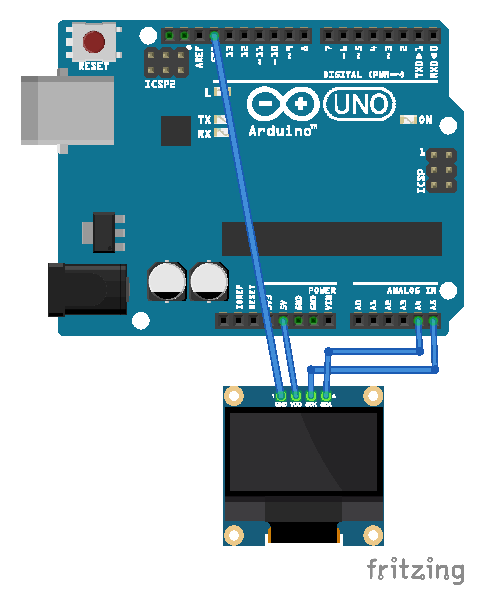
\includegraphics[width=0.6\textwidth]{../3_Chapter3_DISPLAY/Picture/OLED.pdf}
	\caption{显示屏连接}
	\label{fig:显示屏连接}
	\hfill
\end{figure}

\begin{itemize}
	\item 显示器vcc接arduino上的5v;
	\item 显示器Gnd接arduino上的Gnd;
	\item 显示器SCL接arduino上的SCL;
	\item 显示器SDA接arduino上的SDA;
\end{itemize}

主程序中显示器部分:
\begin{lstlisting}
#include "Oled.h"

Oled oled;

void setup() {
  oled.initialize();
}

void loop() {
  oled.show(btn.CalibratedWeight);
}
\end{lstlisting}

其中: oled.initialize()初始化了Oled类中变量, 用Oled类中的成员函数display在OLED屏显示Button类中校准后的读数CalibratedWeight。
具体过程在下一小节。

\subsection{Oled类的声明}

\begin{lstlisting}
class Oled {
private:
  Adafruit_SSD1306 display;
public:
  void initialize();
  void show(unsigned long);
};
\end{lstlisting}

在initialize()中, 实例化Adafruit\_SSD1306类, 128,64分别是OLED屏的宽和高, Wire表示用的I2C通信, 没有设置重置引脚时, 就是-1;并用begin方法初始化,
IIC地址为 0x3C。
\begin{lstlisting}
void Oled::initialize() {
  display = Adafruit_SSD1306(128, 64, &Wire, -1);
  display.begin(SSD1306_SWITCHCAPVCC, 0x3C);
};
\end{lstlisting}

在show(unsigned long)中, 将校准后的读数显示在屏幕如下:
\begin{lstlisting}
void Oled::OLED_show(unsigned long val) {
  display.clearDisplay();

  display.setTextSize(2);
  display.setTextColor(WHITE);

  display.setCursor(20, 10);
  display.print(val);
  display.display();  
};
\end{lstlisting}
分为三步:

\noindent 第一步: display.clearDisplay()清空OLED屏缓存;
\begin{lstlisting}
  display.clearDisplay();
\end{lstlisting}
第二步: setTextSize, setTextColor设置显示的字体大小及颜色;
\begin{lstlisting}
  display.setTextSize(2);
  display.setTextColor(WHITE);  
\end{lstlisting}
第三步: setCursor设置光标开始的位置, prin输入打印内容, display展示到屏幕。
\begin{lstlisting}
  display.setCursor(20, 10);
  display.print(val);
  display.display();  
\end{lstlisting}

\subsection{DISPLAY.ino}
\begin{lstlisting}
  #include "Surface.h"
  #include "Calibrate.h"
  #include "Oled.h"
  
  Surface YL_Surface;
  Calibrate YL_Calibrated;
  Oled oled;
  
  void setup() {
    Serial.begin(9600);
    YL_Calibrated.setpin_SCKDT(4, 5);
    YL_Calibrated.set_range(20);
    YL_Calibrated.kb_Initialize();  
    oled.initialize();
  }
  
  void loop() {
    unsigned long CalibratedWeight = YL_Calibrated.Output_CalibratedWeight(YL_Surface.Get_Surface());
    oled.show(CalibratedWeight);
    delay(1000);
  }  
\end{lstlisting}

主程序基本没什么变化, 就是把数据打印在串口换成打印在OLED屏幕。

\section{第四章: I2C通信}
这里采用IIC通信协议进行不同arduino板之间的通信, 硬件连接很简单, 只需要将arduino上SCL和SDA和其他arduino的相同端口分别连接即可。但为了便于电脑
读取串口数据, 每个板需要单独和电脑用USB数据线连接, 如下图所示。
\begin{figure}[h]
    \centering
    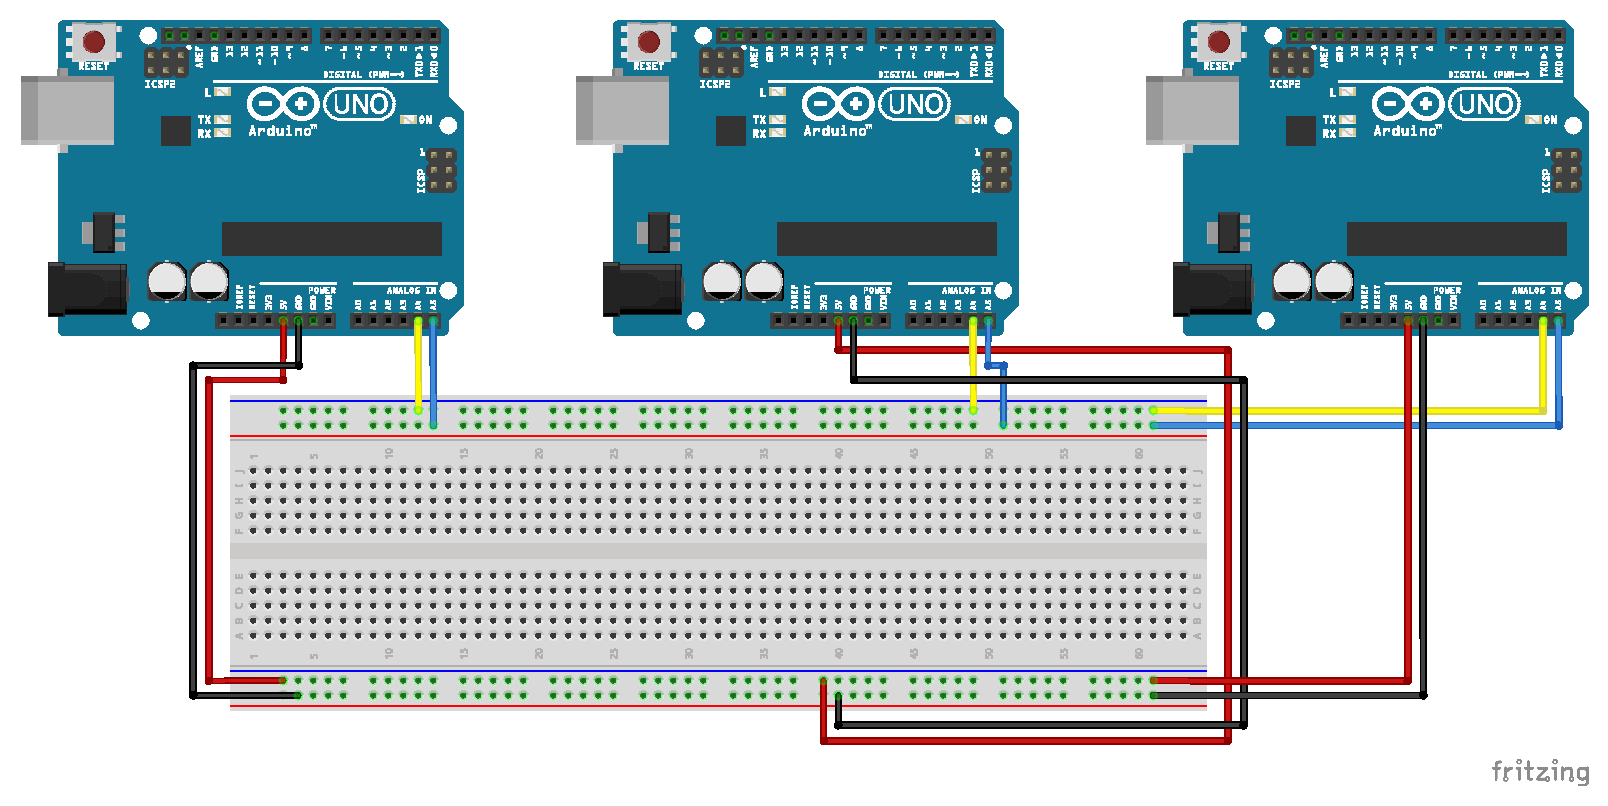
\includegraphics[width=0.6\linewidth]{../4_Chapter4_COMMUNICATION/picture/I2C_.pdf}
    \caption{Wire板间通信电路图}
    \label{fig:Wire板间通信电路图}
\end{figure}

\begin{figure}[h]
     \centering
     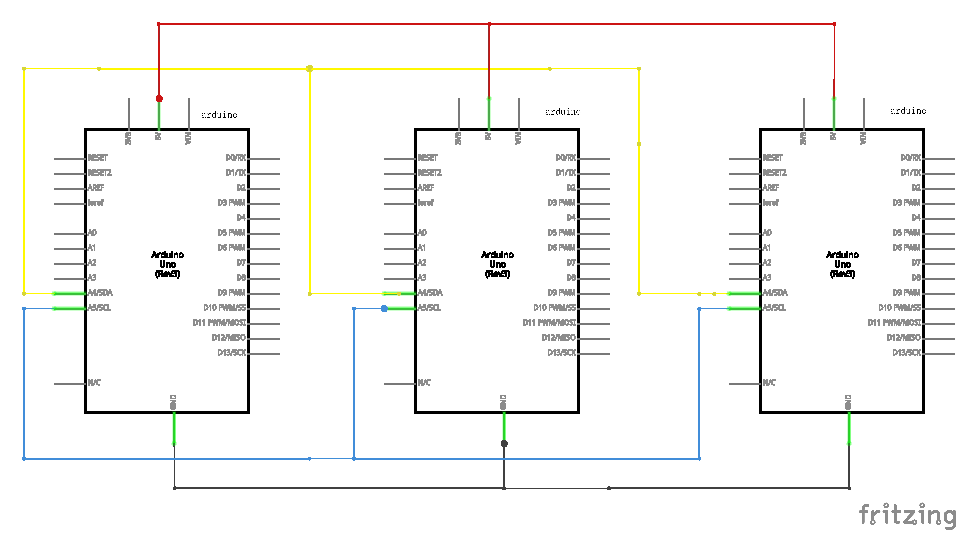
\includegraphics[width=0.6\linewidth]{../4_Chapter4_COMMUNICATION/picture/I2C_line.pdf}
     \caption{Wire板间通讯电路原理图}
     \label{fig:Wire板间通讯电路原理图}
\end{figure}

IIC通信分三步:
\begin{itemize}
    \item 整理等待发送的数据内容;
    \item 确定好主从机地址, 主机向从机发送数据;
    \item 从机接收主机发送过来的内容并做出相应。
\end{itemize}

\subsection{准备发送的消息}
通信时的消息需要按照一定的格式进行整理后发送, 这一节就是介绍整理消息的transform类。
\subsubsection{transform类的声明}
传递的数据包括物品种类、设备地址、物品数量、物品重量这些已知信息。在发送前, 数据按以下格式进行分配处理。

\begin{table}[h]
  \centering
  \begin{tabularx}{\textwidth}{|X|X|X|X|}
    \hline
    物品种类 & 设备IIC通信地址 & 物品数量 & 物品重量  \\
    \hline
    3字节 & 2字节 & 4字节 & 6字节 \\
    \hline
  \end{tabularx}
  \caption{I2C 发送数据格式。}
  \label{tab:example}
\end{table}

其中物品种类由Type\_Name[3]表示, 因为可能会有上千种组合, 所以暂定用三个字节储存; 设备IIC通信地址由DEVICE\_ADDRESS表示; 物品数量由当前称出的物品重量除以单个重量得到。
根据本章开头的需求描述, 创建了一个transform类来打包所有信息到一个字符数组Transmission\_Information。

\begin{lstlisting}
class transform {
private:
  unsigned long Weight;
public:
  char Transmission_Information[15];
  char Type_Name[3];
  long Number;
  int DEVICE_ADDRESS;

  transform();
  void pack(char *Type, int DEVICE, int num, unsigned long W);
  void unpack(String data);
  void show();
};
\end{lstlisting}

\begin{itemize}
  \item 物品种类Type\_Name, 设备IIC通信地址DEVICE\_ADDRESS, 物品数量Number, 物品重量Weight;
  \item 打包后的消息Transmission\_Information;
  \item pack是处理已知信息, 更新字符数组Transmission\_Information, 之后就可以直接发送;
  \item unpack是处理收到的消息, 更新物品种类Type\_Name, 设备IIC通信地址DEVICE\_ADDRESS, 物品数量Number;
  \item show在串口打印字符数组Transmission\_Information。
\end{itemize}

默认构造函数, 因为当没有收到消息时, OLED屏显示的数很奇怪, 所以在默认构造函数里先赋初始值。
\begin{lstlisting}
transform::transform(){
  for(int i=0; i<2; i++) Type_Name[i] = '0';
  DEVICE_ADDRESS = 8;
  Number = 0;
  Weight = 0;
};
\end{lstlisting}

消息打印函数如下:
\begin{lstlisting}
void transform::show() {
  Serial.println(Transmission_Information);
}
\end{lstlisting}

\subsubsection{pack函数和unpack函数}
在主机发消息前, 需要将已知的物品种类Type\_Name, 从机地址DEVICE\_ADDRESS, 物品数量Number, 物品重量Weight整理一个字符数组, 
pack函数就是完成这个转换, 更新transform类的Transmission\_Information。
\begin{lstlisting}
void transform::pack(char *Type, int DEVICE, int num, unsigned long W) {
  for(int i=0; i<2; i++) Type_Name[i] = Type[i];
  DEVICE_ADDRESS = DEVICE;
  Number = num;
  Weight = W;

  Transmission_Information[0] = Type_Name[0];
  Transmission_Information[1] = Type_Name[1];

  if (DEVICE_ADDRESS < 10)
  {
      Transmission_Information[2] = 0 + 48;
      Transmission_Information[3] = DEVICE_ADDRESS + 48;
  }
  else
  {
      Transmission_Information[2] = DEVICE_ADDRESS / 10 + 48;
      Transmission_Information[3] = DEVICE_ADDRESS % 10 + 48;
  }

  if (Number < 0)
  {
      Number = -Number;
      Transmission_Information[4] = 48;
      Transmission_Information[5] = 48;
      Transmission_Information[6] = 48;
      Transmission_Information[7] = 48;
  }
  else
  {
      byte k = 4;
      while (Number / 10 > 0)
      {
          Transmission_Information[k] = (Number % 10) + 48;
          Number = Number / 10;
          ++k;
      }
      for (int i = k; i < 8; ++i)
      {
          Transmission_Information[i] = 48;
      }
      Transmission_Information[k] = Number + 48;
      byte num = 4;
      for (int j = num; j < (8 -3)/2+4; ++j)
      {
          char m = Transmission_Information[j];
          Transmission_Information[j] = Transmission_Information[8-1 - j + num];
          Transmission_Information[8-1 - j + num] = m;
      }
  }
  
  if (Weight < 0)
  {
      Weight = -Weight;
      Transmission_Information[8] = 48;
      Transmission_Information[9] = 48;
      Transmission_Information[10] = 48;
      Transmission_Information[11] = 48;
      Transmission_Information[12] = 48;
      Transmission_Information[13] = 48;
  }
  else
  {
      byte k = 8;
      while (Weight / 10 > 0)
      {
          Transmission_Information[k] = (Weight % 10) + 48;
          Weight = Weight / 10;
          ++k;
      }
      for (int i = k; i < 14; ++i)
      {
          Transmission_Information[i] = 48;
      }
      Transmission_Information[k] = Weight + 48;
      byte num = 8;
      for (int j = num; j < (14 - 8) / 2 + 8; ++j)
      {
          char m = Transmission_Information[j];
          Transmission_Information[j] = Transmission_Information[14-1 - j + num];
          Transmission_Information[14-1 - j + num] = m;
      }
  }
  Transmission_Information[14] = '\0';  
};  
\end{lstlisting}

在从机收到消息后, 需要提取消息中的信息, unpack函数就是提取物品种类Type\_Name, 主机地址DEVICE\_ADDRESS, 物品数量Number并更新
transform类中的相关变量。
\begin{lstlisting}
void transform::unpack(String comdata) {
  for (int i=0; i<2; i++) Type_Name[i]=comdata[i];
  DEVICE_ADDRESS = (comdata[2]-48)*10+comdata[3]-48;
  Number = (comdata[4]-48)*pow(10,3)+(comdata[5]-48)*pow(10,2)+(comdata[6]-48)*pow(10,1)+(comdata[7]-48);
}  
\end{lstlisting}

\subsubsection{transform.ino}
\begin{lstlisting}
#include "transform.h"
#include "Surface.h"
#include "Calibrate.h"

Surface YL_Surface;
Calibrate YL_Calibrated;
transform tf;

char te[3] = {'A','A','\0'}; 
unsigned long Sweight=10;
int address = 10;
long numbefore=0, numnow=1;

void setup() {
  Serial.begin(9600);
  YL_Calibrated.setpin_SCKDT(4, 5);
  YL_Calibrated.set_range(20);
  YL_Calibrated.kb_Initialize();
}

void loop() {
  numbefore = numnow;
  unsigned long CalibratedWeight = YL_Calibrated.Output_CalibratedWeight(YL_Surface.Get_Surface());
  numnow = ceil(CalibratedWeight/Sweight);

  bool flag= (numbefore==numnow?0:1);
  if(flag){
    tf.pack(te, address, numnow, CalibratedWeight);
    tf.show();
  }

  delay(3000);
}
\end{lstlisting}

还是分为三部分:\\
\noindent 1. 实例化Surface, Calibrate, transform类; numbefore是上一次物品数量, 初始化为0, numnow是当前物品数量, 初始化为1; 
te[]是物品种类, 暂定为AA, 在第五章中会通过RFID读到准确值; Sweight是单个物品重量,
用于计算物品数量, 暂定为10, 在第五章中会通过RFID读到准确值; address是设备IIC通信地址, 在下一节会介绍, 暂定为10:
\begin{lstlisting}
Surface YL_Surface;
Calibrate YL_Calibrated;
transform tf;

char te[3] = {'A','A','\0'}; 
unsigned long Sweight=10;
int address = 10;
long numbefore=0, numnow=1;  
\end{lstlisting}

\noindent 2. 和DISPLAY.ino一样设置setup部分:
\begin{lstlisting}
Serial.begin(9600);
YL_Calibrated.setpin_SCKDT(4, 5);
YL_Calibrated.set_range(20);
YL_Calibrated.kb_Initialize(); 
\end{lstlisting}

\noindent 3. 计算校准后的称重结果以及当前物品数量, 如果和上一时刻相比, 物品数量发生了变化, flag就赋值为1,
在if中进行数据打包, 在通过show()打印出打包后的数据:

\begin{lstlisting}
void loop() {
  numbefore = numnow;
  unsigned long CalibratedWeight = YL_Calibrated.Output_CalibratedWeight(YL_Surface.Get_Surface());
  numnow = ceil(CalibratedWeight/Sweight);

  bool flag= (numbefore==numnow?0:1);
  if(flag){
    tf.pack(te, address, numnow, CalibratedWeight);
    tf.show();
  }

  delay(3000);
}
\end{lstlisting}

\subsection{发送打包后的数据}
IIC通信时根据信息发送方向分为主机从机两种, 这里我们把所有arduino板定义为主机, 向上位机直接发送数据。
所以这里创建了一个master类用于arduino的信息发送。

\subsubsection{master类的声明}
master类仅负责数据的发送。
\begin{lstlisting}
class master {
public:
  int address;
  master();
  void initialize(int add);
  void send(int add, char *data);
};
\end{lstlisting}

这里定义了三个函数。
\begin{lstlisting}
master::master(){};  
\end{lstlisting}

initialize用于设置IIC通信地址, 并更新master类中的address:
\begin{lstlisting}
void master::initialize(int add) {
  address=add;
  Wire.begin(add);
}; 
\end{lstlisting}

send用于传入接收方地址add, 发送的字符数组data:
\begin{lstlisting}
void master::send(int add, char *data) {
  Wire.beginTransmission(add);
  Wire.write(data);
  Wire.endTransmission(add);
};
\end{lstlisting}

\subsubsection{master.ino}
在上一节transform.ino的基础上, 加入了master类, 发送的数据就是字符数组Transmission\_Information。发送方地址为10, 接收方地址为8。
\begin{lstlisting}
#include "master.h"
#include "transform.h"
#include "Surface.h"
#include "Calibrate.h"
#include "Oled.h"

master m1;
Surface YL_Surface;
Calibrate YL_Calibrated;
transform tf;
Oled oled;

long numbefore=0, numnow=1;
char te[3] = {'A','A','\0'}; 
unsigned long Sweight=10;

void setup() {
  Serial.begin(9600);
  m1.initialize(10);   
  YL_Calibrated.setpin_SCKDT(4, 5);
  YL_Calibrated.set_range(20);
  YL_Calibrated.kb_Initialize();
  oled.initialize();
  pinMode(3, OUTPUT);
  digitalWrite(3, LOW);
}

void loop() {
  numbefore = numnow;
  unsigned long CalibratedWeight = YL_Calibrated.Output_CalibratedWeight(YL_Surface.Get_Surface());
  numnow = ceil(CalibratedWeight/Sweight);

  bool flag= (numbefore==numnow?0:1);
  if(flag){
    tf.pack(te, m1.address, numnow, CalibratedWeight);
    m1.send(8, tf.Transmission_Information);
    Serial.println(tf.Transmission_Information);
    oled.showIIC(te, numnow);
  }

  delay(3000);
}
\end{lstlisting}

在Oled类中新加了一个showIIC函数。屏幕显示格式为“物品种类:物品数量”:
\begin{lstlisting}
void Oled::showIIC(char *type, int num) {
  display.clearDisplay(); // 清除屏幕

  //设置字体大小 设置字体颜色,白色可见
  display.setTextSize(4);
  display.setTextColor(WHITE);

  //设置光标位置 
  display.setCursor(5, 10);
  display.print(type[0]);
  display.print(type[1]);
  display.print(":");
  display.print(num);
  display.display(); 
}  
\end{lstlisting}

\subsubsection{slave类的声明}
slave类负责接收数据并打印在串口。
\begin{lstlisting}
class slave{
public:
  static  String comdata;

  slave();
  void initialize(int add);
static void receiveEvent(int howmany);};  
\end{lstlisting}

由于IIC从机的响应事件函数在内中必须是无返回值的静态函数, 所以为了方便在响应事件读完数据后, 直接得到一个字符串便于transform类中的unpack函数操作, 
故将得到的字符串comdata设为静态成员变量。

\begin{lstlisting}
slave::slave(){};  
\end{lstlisting}

initialize设置从机通信地址, 并注册接收事件, 即在接收到主机发送的信息后要执行的事件。
\begin{lstlisting}
void slave::initialize(int add){
  Wire.begin(add);
  Wire.onReceive(receiveEvent);
};  
\end{lstlisting}

receiveEvent传入的参数没有用到, 是代码格式要求。通过判断是否IIC线上有消息可读, 来对buffer进行填充, 写完后再一一写入字符串comdata, 最终comdata在串口
打印出来。
\begin{lstlisting}
void slave::receiveEvent(int howmany){
  String buffer="";
  while(Wire.available()) {
    buffer += (char) Wire.read();
  }
  comdata = "";
  for (char i:buffer) comdata+=i;
  Serial.print("comdata:");
  Serial.println(comdata);
};  
\end{lstlisting}

\subsubsection{slave.ino}
实现的就是从机接收到后解包, 更新transform类中的物品种类Type\_Name, 设备IIC通信地址DEVICE\_ADDRESS, 物品数量Number。
\begin{lstlisting}
#include "slave.h"
#include "transform.h"

String slave::comdata="";

slave s;
transform tf;

void setup() {
  Serial.begin(9600);
  s.initialize(8);
}

void loop() {
  tf.unpack(s.comdata);
  delay(1000);
}
\end{lstlisting}

\subsection{上位机对I2C数据的读取}
上位机通过python读取arduino在串口中打印的信息。
\lstinputlisting{../4_Chapter4_COMMUNICATION/TEX/code/uppermachine.txt}

\subsection{驱动多路OLED}
考虑到一个货架上摆放多个秤时, 如果所有秤的OLED屏是直接连在arduino板上, 不同的arduino板之间也直接用I2C通信的话, 那么所有的OLED屏则会显示相同的内容, 更麻烦的是, 在不同arduino板
要显示的内容不一样时, OLED屏会因为反复清楚屏幕和打印内容到屏幕而导致屏幕闪烁。所以我们需要一个额外的器件控制OLED屏的分配。这里有两套方案。
\begin{itemize}
  \item TCA9548A模块连接一个arudino板作为从机接收所有arduino板发送过来的消息, 然后分别打印在TCA9548A连接的其中一个OLED屏;
  \item CMOS元件控制是否打开arduino和OLED屏之间的通信, 在没有新消息的时候就关闭连接, 有新消息的时候就打开连接。
\end{itemize}

\subsubsection{TCA9548A}
\begin{figure}[h]
  \centering
  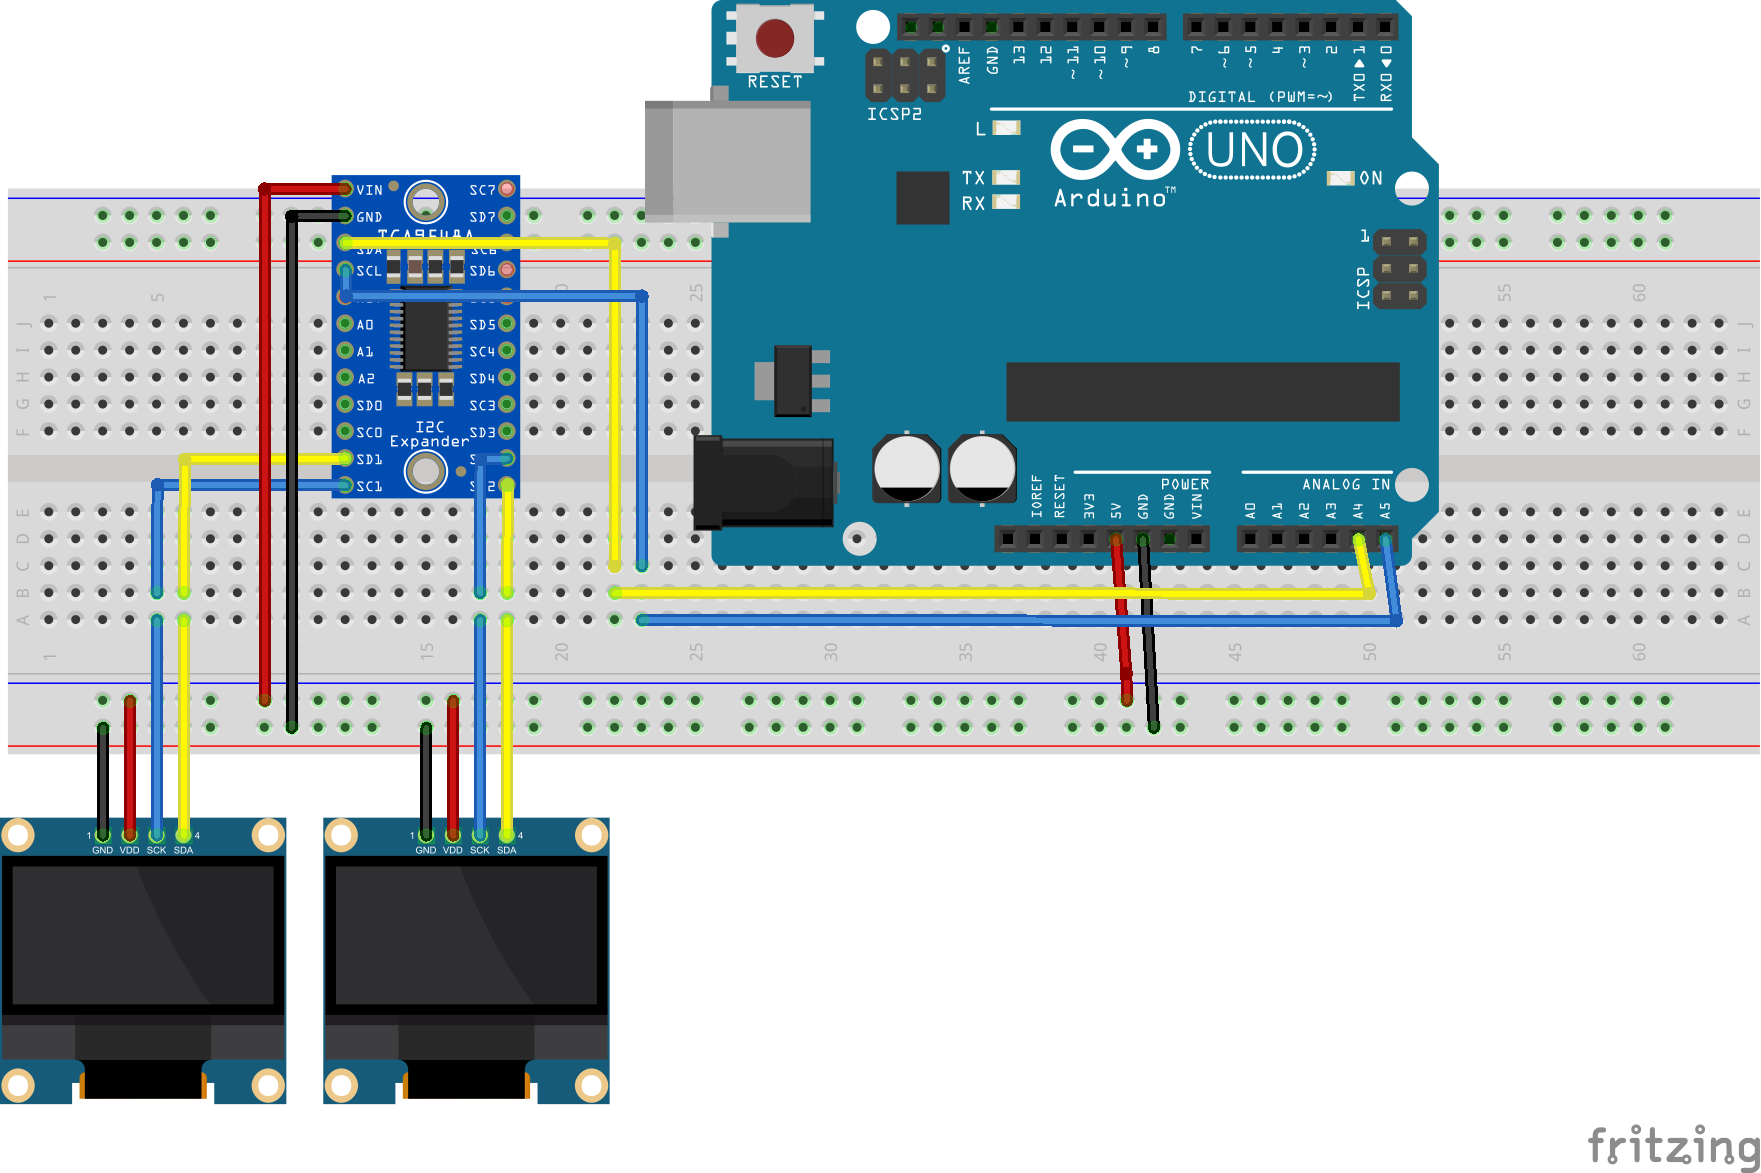
\includegraphics[width=0.6\textwidth]{../4_Chapter4_COMMUNICATION/Picture/TCA9548A.png}
  \caption{TCA9548A电路图}
  \label{fig:TCA9548A电路图}
\end{figure}

TCA9548A 器件配有八个可通过 I2C 总线控制的双向转换开关。串行时钟/串行数据 (SCL/SDA) 上行对可扩展为 8 个下行对或通道。根据可编程控制寄存器的内容,
可选择任一单独 SCLn/SDAn 通道或者通道组合。这些下游通道可用于解决 I2C 从器件地址冲突。例如,如果应用中需要八个完全相同的数字温度传感器,
则每个通道(0-7)可以连接一个传感器。

\begin{figure}[h]
  \centering
  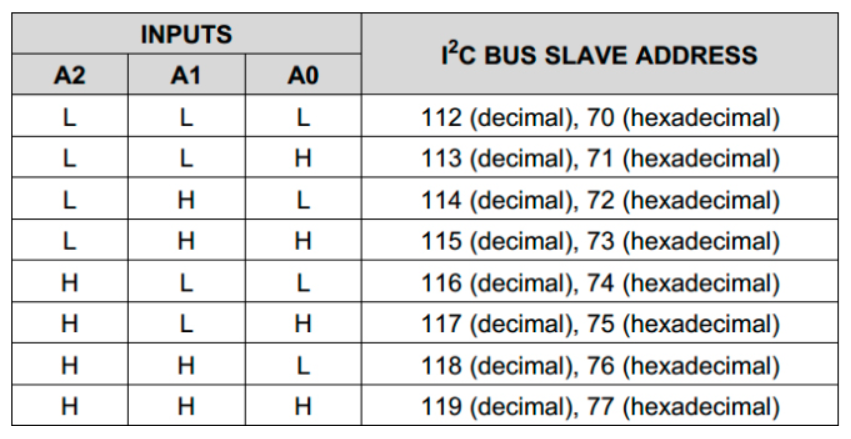
\includegraphics[width=0.6\textwidth]{../4_Chapter4_COMMUNICATION/Picture/tcai2c.png}
  \caption{TCA9548A地址和电平状态}
  \label{fig:TCA9548A地址和电平状态}
\end{figure}

TCA9548A 是一个I2C器件,本身有I2C地址。TCA9548A自身的地址和它A0, A1, A2的电平状态有关, 总共可以组合出8个I2C地址。默认地址为0x70(A0,A1, A2全部接地), 
最大地址为0x77(A0,A1,A2全部上拉)。而对于固定地址的TCA9548A, 通过移位的操作, 可以选择消息输出到OLED的通道, 具体来说就是:

\begin{lstlisting}
class Oled {
private:
  Adafruit_SSD1306 display;
public:
  void initialize();
  void showIIC(char *type, int num, int i);
};
\end{lstlisting}

initialize函数没有变化
\begin{lstlisting}
void Oled::initialize() {
  display = Adafruit_SSD1306(128, 64, &Wire, -1);
  display.begin(SSD1306_SWITCHCAPVCC, 0x3C);
};  
\end{lstlisting}

showIIC中传入的参数加入了address, 在IIC通信中的Wire.write下, 9号发消息的主机对应的是TCA9548A的SD0,SC0通道, 10号对应是SD1,SC1通道, 以此类推, 
最多可以用8个通道, 用哪个通道就往哪个通道发消息。
\begin{lstlisting}
void Oled::showIIC(char *type, int num, int address) {
  Wire.beginTransmission(0x70);
  Wire.write(1<<(address-9));
  Wire.endTransmission();
  display.clearDisplay(); // 清除屏幕

  //设置字体大小 设置字体颜色,白色可见
  display.setTextSize(2);
  display.setTextColor(WHITE);

  //设置光标位置 
  display.setCursor(5, 10);
  display.print(type[0]);
  display.print(type[1]);
  display.print(":");
  display.print(num);
  display.display(); 
};
\end{lstlisting}

\subsubsection{TCA9548A.ino}
与TCA9548A相连的arduino板上的主程序如下
\begin{lstlisting}
#include "Oled.h"
#include "slave.h"
#include "transform.h"

String slave::comdata="";

Oled oled;
slave s;
transform tf;

void setup() {
  Serial.begin(9600);
  s.initialize(8);
  oled.initialize();
  pinMode(7,INPUT);
  digitalWrite(7, LOW);
}

void loop() {
  tf.unpack(s.comdata);
  oled.showIIC(tf.Type_Name, tf.Number, tf.DEVICE_ADDRESS);
  delay(1000);
}
\end{lstlisting}
首先初始化了slave类中的静态变量, comdata在slave中的响应事件里更新, 这里选择将数字引脚7连接到TCA9548A中的复位引脚, 当写入低电平时可以复位,
使得屏幕在卡住的时候也能重新显示。然后通过Oled中的showIIC在DEVICE\_ADDRESS对应的Oled屏上打印消息。

\subsubsection{一层货架示意图}
假设现在每一层有三个电子秤, 如果采取TCA9548A的显示屏连接方案, 则还需要另一个arduino板作为从机接收所有电子秤发送过来的消息, 并判断在对应
位置的显示屏显示对应的数据。

\begin{figure}[h]
  \centering
  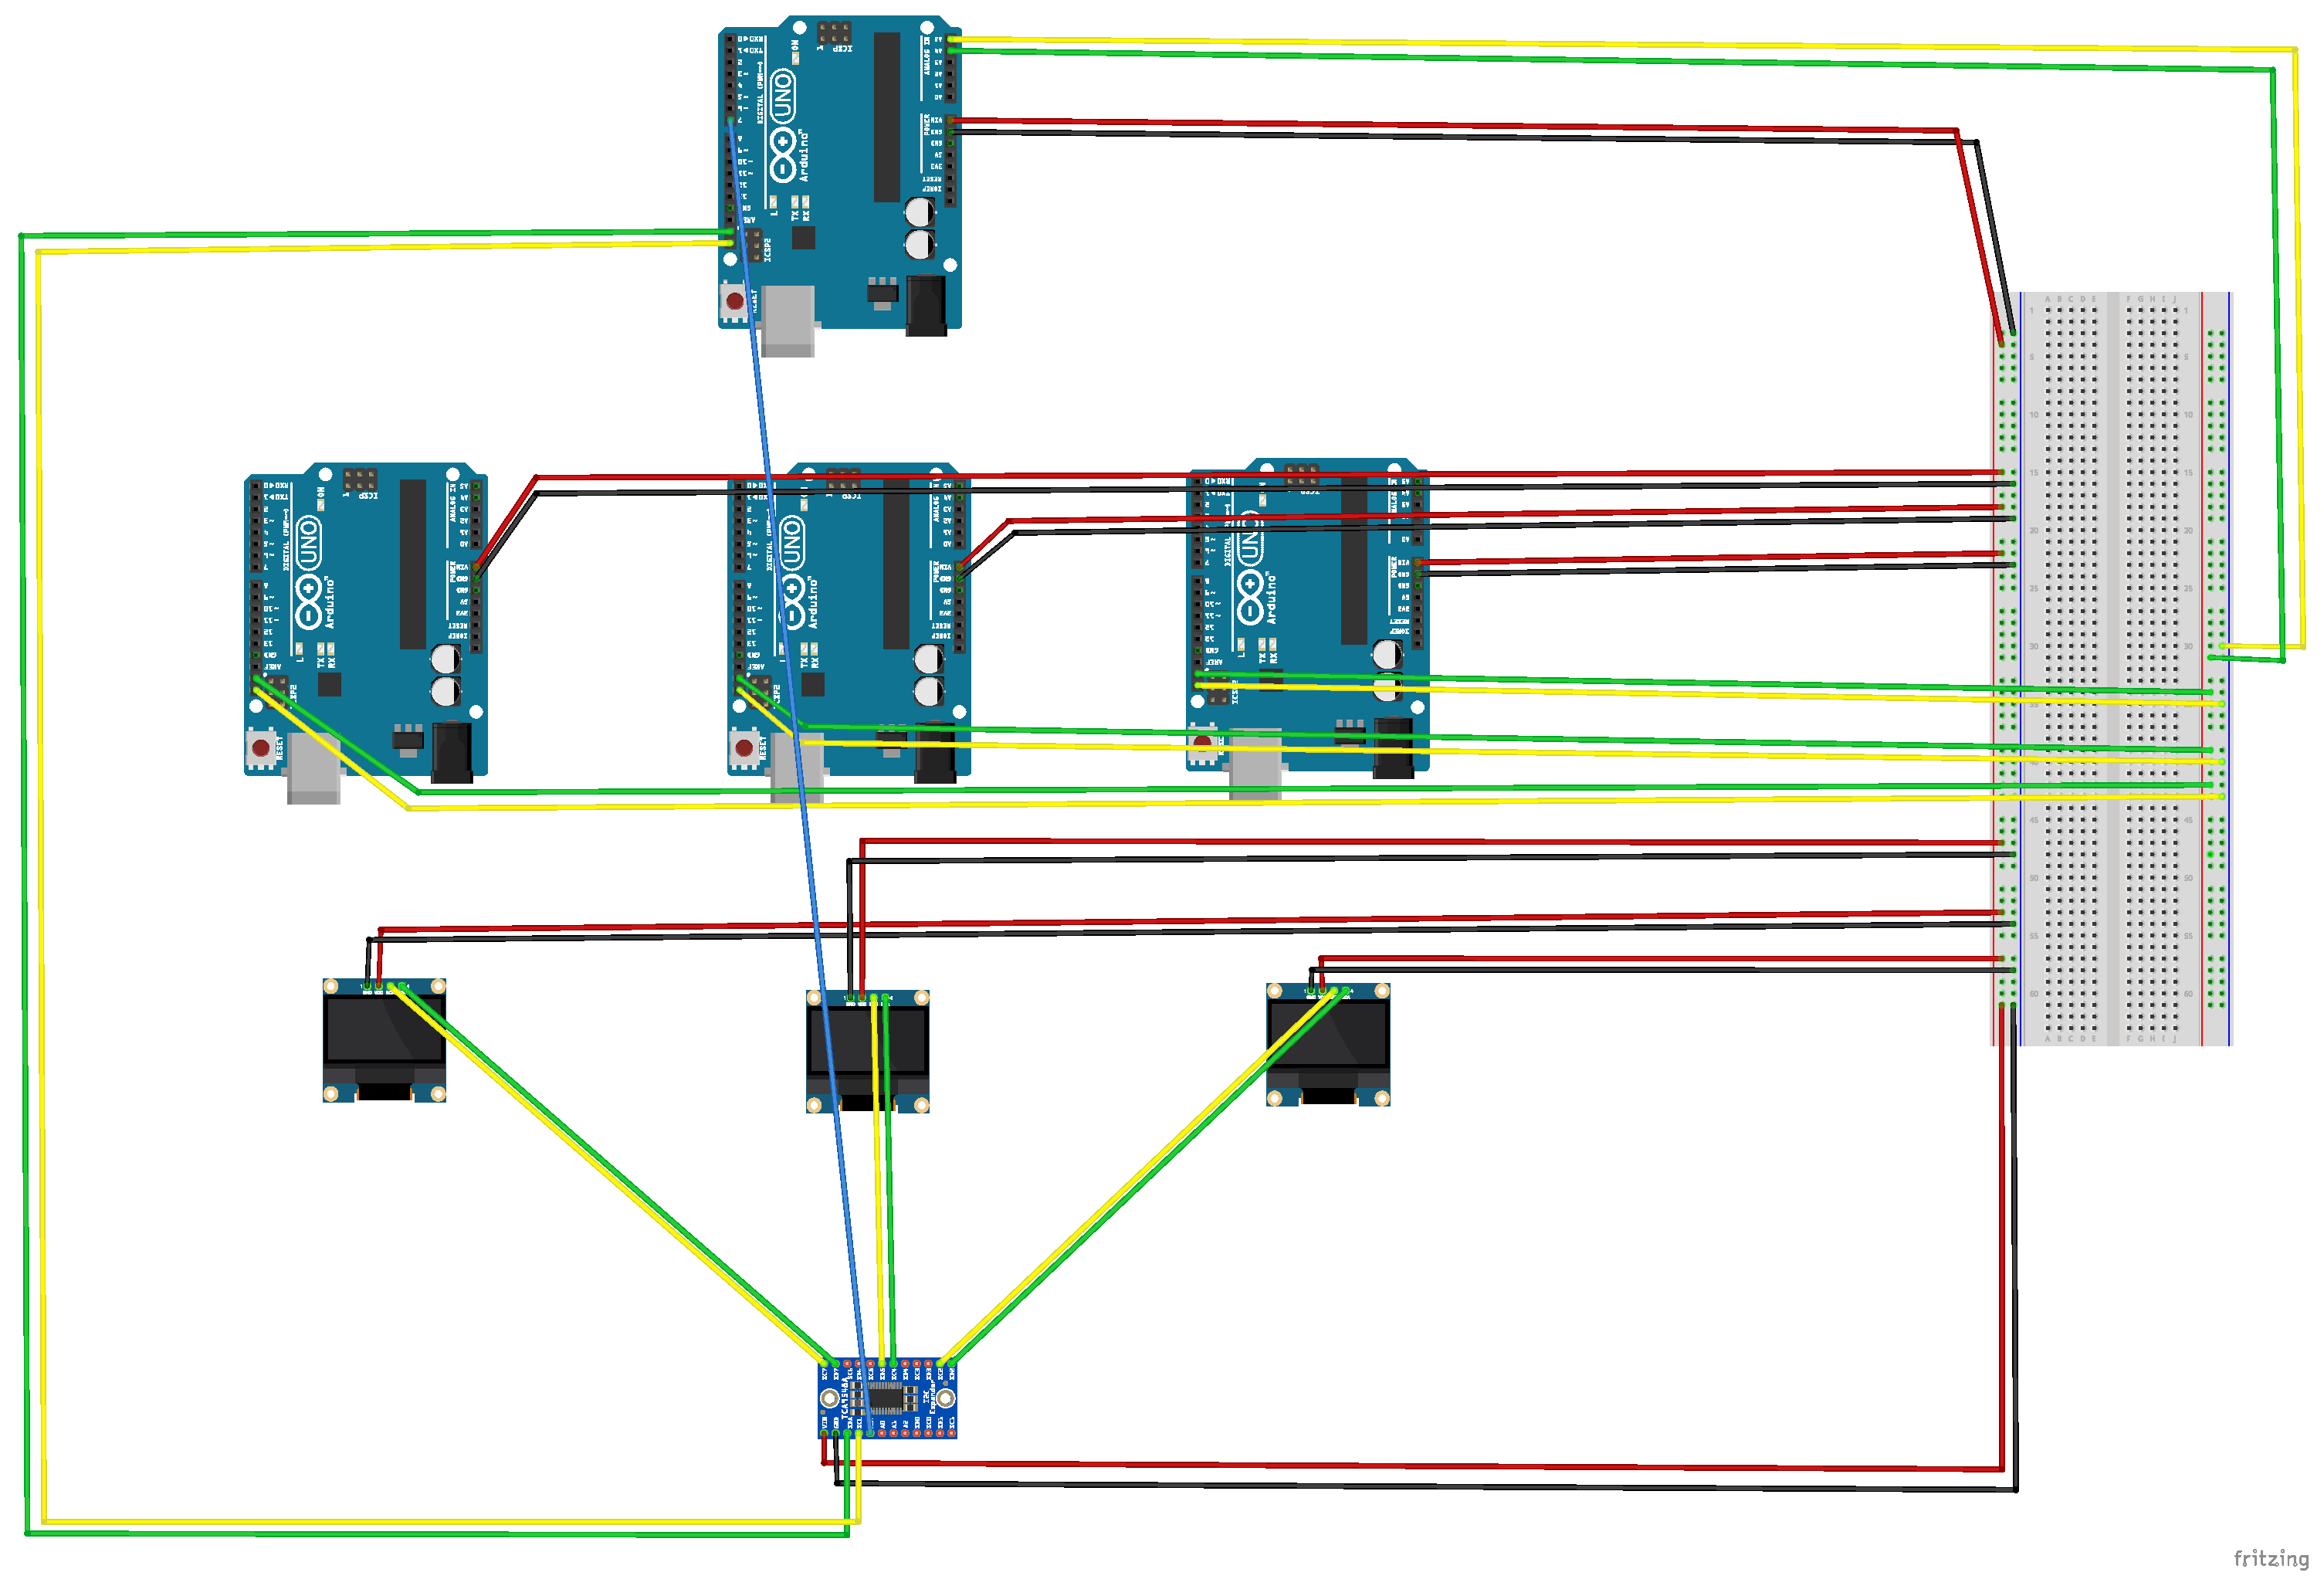
\includegraphics[width=0.8\textwidth]{../4_Chapter4_COMMUNICATION/Picture/一层货架示意图.pdf}
  \caption{一层货架示意图}
  \label{fig:一层货架示意图}
\end{figure}

如图所示, 三个OLED屏对应三个arduino板, 连接时主要四条主线, 分别是5V的红线, 接地的黑线, SDA的绿线, SCL的黄线。其中需要注意的是, OLED屏不能
与对应位置的arduino板直接相连, 因为OLED屏本身没有地址分配, 无法指定显示特定内容, 需要借助TCA9548A, 通过选择通道0到7来选择在哪一个OLED屏上
显示哪一个板的内容。

\subsubsection{MOS}
MOS是通过选择性接通某一个arduino对应的OLED屏来避免该OLED屏总接收到其他arduino板的消息, 来避免显示错误, 就相当于一个开关。
\begin{figure}[h]
  \centering
  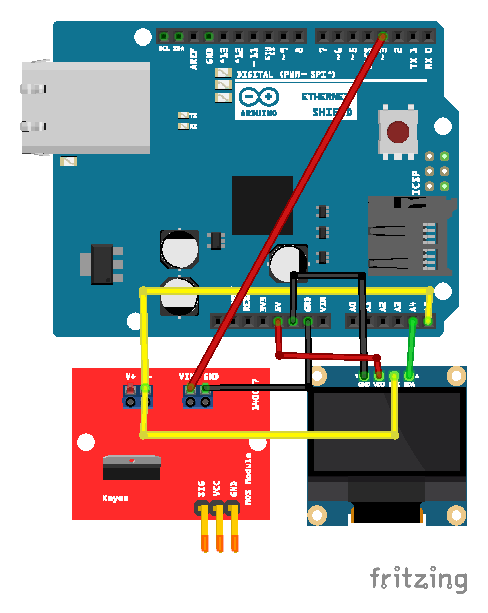
\includegraphics[width=0.4\textwidth]{../4_Chapter4_COMMUNICATION/Picture/MOS.pdf}
  \caption{MOS连接图}
  \label{fig:MOS连接图}
\end{figure}

\subsubsection{MOS.ino}
和TCA9548A.ino相比, 加入了数字引脚3, 来控制MOS的电平写入, 在comdata不为空字符串时, 改变3号引脚, 如果pinMode时设置的是输入模式,
则写入高电平时接通OLED和arduino, 如果是输出模式, 则是写入低电平时接通OLED和arduino。
\begin{lstlisting}
#include "Oled.h"
#include "slave.h"
#include "transform.h"

String slave::comdata="";

Oled oled;
slave s;
transform tf;

void setup() {
  Serial.begin(9600);
  s.initialize(8);
  oled.initialize();
  pinMode(3,INPUT);
}

void loop() {
  if (s.comdata!=""){
    tf.unpack(s.comdata);
    s.comdata="";
    digitalWrite(3, HIGH);  
    oled.show(tf.Type_Name, tf.Number, tf.DEVICE_ADDRESS);
    digitalWrite(3,LOW);
  }
  delay(1000);
}


\end{lstlisting}

\section{第五章: 射频识别技术(RFID-RC522)}
在上一章中, 我们是直接给的物品种类以及单个物品质量的信息。实际上这是从RC522读卡器上的卡读到的。首先来认识RC522模块,
\begin{figure}[h]
	\centering
	\begin{minipage}{.45\textwidth}
		\centering
		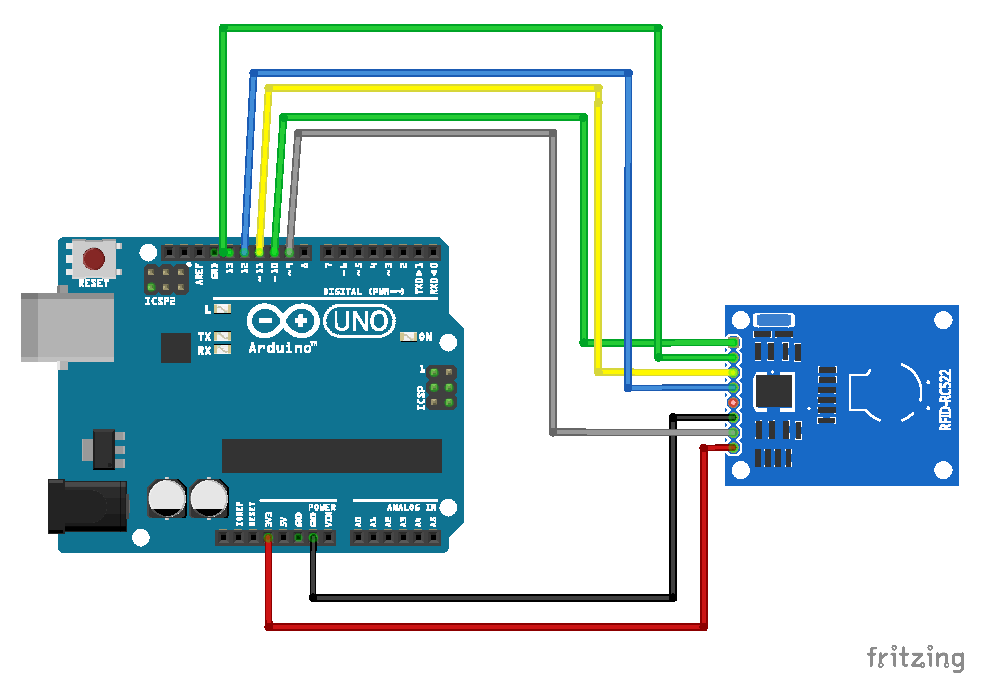
\includegraphics[width=\linewidth]{../5_Chapter5_RC522/Picture/RFID_RC522.pdf}
		\caption{RC522硬件连接}
		\label{fig:RC522硬件连接}
	\end{minipage}%
	\hfill
	\begin{minipage}{.45\textwidth}
		\centering
		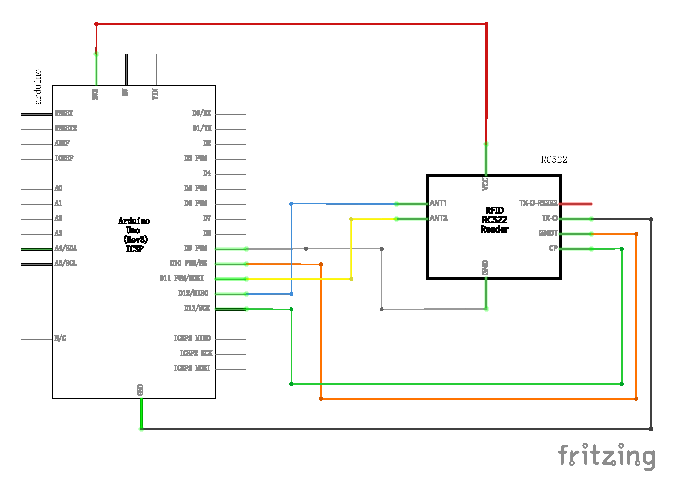
\includegraphics[width=\linewidth]{../5_Chapter5_RC522/Picture/RFID_RC522_line.pdf}
		\caption{RC522连接示意图}
		\label{fig:RC522连接示意图}
	\end{minipage}
\end{figure}

RC522模块共有8个与外界连接的引脚,与arduino的连接如图所示:

\begin{itemize}
	\item VCC为模块供电, 连接到Arduino的3.3V输出。;
	\item RST是复位和掉电的输入。当该引脚变为低电平时,关闭所有内部电流吸收器,包括振荡器,并且输入引脚与外界断开连接。在上升沿,模块被重置;
	\item GND是接地引脚,连接到Arduino的GND引脚;
	\item IRQ是一个中断引脚,可在RFID标签进入附近时向微控制器发出警报;
	\item 当使用SPI接线时, MISO上的数据从从机输出到主机;
	\item 当使用SPI接线时, MOSI上的数据从主机输出到从机;
	\item SCK是串行时钟信号, 由主机产生发送给从机;
	\item ss上信号由主机发送, 以控制与哪个从机通信, 通常是低电平有效信号。
\end{itemize}

在MFRC522模块上只有两个引脚RST和SS可以自己定义,这里将其定义为引脚9和引脚10(除了引脚11, 引脚12, 引脚13外的任意空闲数字引脚皆可, 引脚11,12,13
已经与RC522的引脚MOSI,MISO,SPI连接。将其定义为引脚9和引脚10是常见布局)。

\subsection{RC522类的声明}
RC522类就对应了整个RC522模块的功能。
\begin{lstlisting}
class RC522{
private:
  int RST_PIN, SS_PIN;
  MFRC522 mfrc522;                                           

public:
  char Type_Name[3];  
  long Single_Weight;
  long Shell_Weight;

  RC522();
  void initialize(int p1, int p2);
  byte read();
  bool write();
}	
\end{lstlisting}

\begin{itemize}
	\item 私有变量: RST\_PIN, SS\_PIN分别是与RC522的RST,SS连接的arduino引脚;
	\item 公共变量: Type\_Name, Single\_Weight, Shell\_Weight是储存从读卡器中读到的物品种类, 单个物品质量, 每一层物品质量;
\end{itemize}

默认构造函数:
\begin{lstlisting}
RC522::RC522(){};	
\end{lstlisting}

初始化函数用于引脚的赋值, 初始化SPI通信, 初始化MFRC522类。
\begin{lstlisting}
void RC522::initialize(int p1, int p2){
  RST_PIN=p1;
  SS_PIN=p2;
  SPI.begin();
  mfrc522 = MFRC522(SS_PIN, RST_PIN);                                           
  mfrc522.PCD_Init();  
};	
\end{lstlisting}

\subsection{读卡模式}
将下述代码烧录运行,就做好了读卡准备。
\begin{lstlisting}
byte RC522::read(){
  // init the read state
  byte read_state = 0;
  //default key 
  MFRC522::MIFARE_Key key;
  for (byte i = 0; i < 6; ++i) key.keyByte[i] = 0xFF;
  //some variables we need
  byte block;
  byte len;
  MFRC522::StatusCode status;
  //-------------------------------------------
  // Reset the loop if no new card present on the sensor/reader. This saves the entire process when idle.
  if ( ! mfrc522.PICC_IsNewCardPresent()) {
    return read_state;
  }
  // Select one of the cards
  if ( ! mfrc522.PICC_ReadCardSerial()) {
    return read_state ;
  }
  // read one card
  read_state = 1;
  Serial.println(F("**Card Detected:**"));
  //-------------------------------------------
  // mfrc522.PICC_DumpDetailsToSerial(&(mfrc522.uid)); //dump some details about the card
  // mfrc522.PICC_DumpToSerial(&(mfrc522.uid));      //uncomment this to see all blocks in hex
  //-------------------------------------------

  byte buffer1[18];
  block = 1;
  len = 18;
  //------------------------------------------- GET TYPE NAME
  status = mfrc522.PCD_Authenticate(MFRC522::PICC_CMD_MF_AUTH_KEY_A, block, &key, &(mfrc522.uid)); //line 834 of MFRC522.cpp file
  if (status != MFRC522::STATUS_OK) {
    Serial.print(F("Authentication failed: "));
    Serial.println(mfrc522.GetStatusCodeName(status));
    return read_state;
  }
  status = mfrc522.MIFARE_Read(block, buffer1, &len);
  if (status != MFRC522::STATUS_OK) {
    Serial.print(F("Reading failed: "));
    Serial.println(mfrc522.GetStatusCodeName(status));
    return read_state;
  }
  //PRINT TYPE NAME
  Type_Name[0] = buffer1[0];
  Type_Name[1] = buffer1[1];
  long singleweight = 0;
  for (uint8_t i = 2; i < 6; ++i)
  {
    singleweight = singleweight*10 + (buffer1[i]-48);
  }
  Single_Weight = singleweight;
  Serial.print(F("Type Name: "));
  Serial.println(Type_Name);
  Serial.print(F("Type Single Weight: "));
  Serial.println(Single_Weight);
  //---------------------------------------- GET WEIGHT

  byte buffer2[18];
  block = 4;
  status = mfrc522.PCD_Authenticate(MFRC522::PICC_CMD_MF_AUTH_KEY_A, block, &key, &(mfrc522.uid)); //line 834
  if (status != MFRC522::STATUS_OK) {
    Serial.print(F("Authentication failed: "));
    Serial.println(mfrc522.GetStatusCodeName(status));
    return read_state;
  }
  status = mfrc522.MIFARE_Read(block, buffer2, &len);
  if (status != MFRC522::STATUS_OK) {
    Serial.print(F("Reading failed: "));
    Serial.println(mfrc522.GetStatusCodeName(status));
    return read_state;
  }
  //PRINT WEIGHT
  int shellweight = 0;
  for (uint8_t i = 1; i < 16; ++i) {
    // Serial.write(buffer2[i] );
    // Serial.println();
    // Serial.println(buffer2[i]);
    if(buffer2[i] == 32) break;
    shellweight =   shellweight*10 + (buffer2[i]-48);
  }
  Shell_Weight = shellweight;
  Serial.print(F("Shell Weight: "));
  Serial.println(Shell_Weight);
  //----------------------------------------
  Serial.println(F("**End Reading**\n"));
  read_state = 2;
  mfrc522.PICC_HaltA();
  mfrc522.PCD_StopCrypto1();
  return read_state;
}
\end{lstlisting}

\subsection{写卡模式}
将下述代码烧录运行,就做好了写卡准备。写卡时会在串口提示输入两次字符串, 每次都是以\#结尾。第一次是输入物品种类以及单个物品质量, 例如'AA0010\#'表示
物品种类是'AA',单个物品质量是10g;第二次是输入外壳质量, 例如'0\#'表示外壳质量是0。
\begin{lstlisting}
bool RC522::write(){
  //初始化读卡状态
  //未读到卡为0,读到卡为1
  bool write_state = 0;
  //创建访问密钥,用于验证并访问 MIFARE Classic RFID标签
  //这里用默认卡密钥
  MFRC522::MIFARE_Key key;
  for (byte i = 0; i < 6; i++) key.keyByte[i] = 0xFF;

  //block为卡的不同区域编号
  //len3为读到的字节数
  //status为判断对卡操作是否成功完成的状态变量
  byte block;
  byte len3;
  MFRC522::StatusCode status;

  // 如果传感器/读卡器上没有新卡,则复位循环。这可以在空闲时保存整个进程。
  if ( ! mfrc522.PICC_IsNewCardPresent()) {
    return write_state;
  }

  // 选择一张卡片进行读取
  if ( ! mfrc522.PICC_ReadCardSerial()) {
    return write_state;
  }

  Serial.println(F("**Card Detected:**"));
  // 成功读取到卡片,将读卡状态设为1
  write_state = 1;
  
  //打印UID编号
  Serial.print(F("Card UID:"));    
  for (byte i = 0; i < mfrc522.uid.size; i++) {
    Serial.print(mfrc522.uid.uidByte[i] < 0x10 ? " 0" : " ");
    Serial.print(mfrc522.uid.uidByte[i], HEX);
  }
  //打印PICC类型
  Serial.print(F(" PICC type: "));   
  MFRC522::PICC_Type piccType = mfrc522.PICC_GetType(mfrc522.uid.sak);
  Serial.println(mfrc522.PICC_GetTypeName(piccType));  

  byte buffer3[34];
  //等待20秒从串口输入
  Serial.setTimeout(20000L) ;     
  // 提示:输入类型名称
  Serial.println(F("Type name, ending with #"));
  //从串口读入类型名称到buffer3,len为写入字节长度
  len3 = Serial.readBytesUntil('#', (char *) buffer3, 30) ; 
  // 将未满字节用空格填补
  for (byte i = len3; i < 30; i++) buffer3[i] = ' ';     

  block = 1;
  //选择读取区域和密钥进行身份验证,验证失败打印错误信息并提前终止
  status = mfrc522.PCD_Authenticate(MFRC522::PICC_CMD_MF_AUTH_KEY_A, block, &key, &(mfrc522.uid));
  if (status != MFRC522::STATUS_OK) {
    Serial.print(F("PCD_Authenticate() failed: "));
    Serial.println(mfrc522.GetStatusCodeName(status));
    return write_state;
  }
  else Serial.println(F("PCD_Authenticate() success: "));

  // 对前述验证成功的区域内的信息写入字节数组,写入失败打印错误信息并提前终止
  status = mfrc522.MIFARE_Write(block, buffer3, 16);
  if (status != MFRC522::STATUS_OK) {
    Serial.print(F("MIFARE_Write() failed: "));
    Serial.println(mfrc522.GetStatusCodeName(status));
    return write_state;
  }
  else Serial.println(F("MIFARE_Write() success: "));

  block = 2;
  //选择读取区域和密钥进行身份验证,验证失败打印错误信息并提前终止
  status = mfrc522.PCD_Authenticate(MFRC522::PICC_CMD_MF_AUTH_KEY_A, block, &key, &(mfrc522.uid));
  if (status != MFRC522::STATUS_OK) {
    Serial.print(F("PCD_Authenticate() failed: "));
    Serial.println(mfrc522.GetStatusCodeName(status));
    return write_state;
  }

  // 对前述验证成功的区域内的信息写入字节数组的地址,写入失败打印错误信息并提前终止
  status = mfrc522.MIFARE_Write(block, &buffer3[16], 16);
  if (status != MFRC522::STATUS_OK) {
    Serial.print(F("MIFARE_Write() failed: "));
    Serial.println(mfrc522.GetStatusCodeName(status));
    return write_state;
  }
  else Serial.println(F("MIFARE_Write() success: "));

  byte buffer4[34];
  byte len4;
  // Ask personal data: First name
  Serial.println(F("Type Weight, ending with #"));
  len4 = Serial.readBytesUntil('#', (char *) buffer4, 20) ; // read first name from serial
  for (byte i = len4; i < 20; i++) buffer4[i] = ' ';     // pad with spaces

  block = 4;
  //选择读取区域和密钥进行身份验证,验证失败打印错误信息并提前终止
  status = mfrc522.PCD_Authenticate(MFRC522::PICC_CMD_MF_AUTH_KEY_A, block, &key, &(mfrc522.uid));
  if (status != MFRC522::STATUS_OK) {
    Serial.print(F("PCD_Authenticate() failed: "));
    Serial.println(mfrc522.GetStatusCodeName(status));
    return write_state;
  }

  // 对前述验证成功的区域内的信息写入字节数组,写入失败打印错误信息并提前终止
  status = mfrc522.MIFARE_Write(block, buffer4, 16);
  if (status != MFRC522::STATUS_OK) {
    Serial.print(F("MIFARE_Write() failed: "));
    Serial.println(mfrc522.GetStatusCodeName(status));
    return write_state;
  }
  else Serial.println(F("MIFARE_Write() success: "));

  block = 5;
  //选择读取区域和密钥进行身份验证,验证失败打印错误信息并提前终止
  status = mfrc522.PCD_Authenticate(MFRC522::PICC_CMD_MF_AUTH_KEY_A, block, &key, &(mfrc522.uid));
  if (status != MFRC522::STATUS_OK) {
    Serial.print(F("PCD_Authenticate() failed: "));
    Serial.println(mfrc522.GetStatusCodeName(status));
    return write_state;
  }

  // 对前述验证成功的区域内的信息写入字节数组的地址,写入失败打印错误信息并提前终止
  status = mfrc522.MIFARE_Write(block, &buffer4[16], 16);
  if (status != MFRC522::STATUS_OK) {
    Serial.print(F("MIFARE_Write() failed: "));
    Serial.println(mfrc522.GetStatusCodeName(status));
    return write_state;
  }
  else Serial.println(F("MIFARE_Write() success: "));
  delay(1000); 

  //--------------成功完成读取----------------
  Serial.println(F("\n**End Reading**\n"));
  //停止响应当前正在运行的命令。
    //将 RFID 卡片置于休眠状态,以便进行下一个命令的执行。
  mfrc522.PICC_HaltA();
  //停止当前正在进行的加密。如果 RFID 模块正在与 RFID 卡片进行加密通信,
  //则此代码将停止加密,并将模块置于初始状态,以便进行下一个操作。
  mfrc522.PCD_StopCrypto1();
  //返回写卡状态
  return write_state;
}
\end{lstlisting}

\subsection{RC522.ino}
在上一章master.ino基础上, 加入了通过读卡获得rc522的Single\_Weight和Type\_Name。并通过rflag是否为1判断是读还是写。目前有一点不妥的是, 当没有读到卡时, 在switch语句中
会一直在while中循环直到读到卡。也就是说即使物品总质量发生变化, 也只有在重新放卡后才能发送消息到上位机, 要不然出不了while循环语句。
\begin{lstlisting}
  #include "master.h"
  #include "transform.h"
  #include "Surface.h"
  #include "Calibrate.h"
  #include "Oled.h"
  #include "RC522.h"
  
  master m1;
  Surface YL_Surface;
  Calibrate YL_Calibrated;
  transform tf;
  Oled oled;
  RC522 rc522;
  
  long numbefore=0, numnow=1;
  char te[3];
  unsigned long Sweight;
  bool rflag=1;  //1 ---> read; 0 ---> write
  
  void setup() {
    Serial.begin(9600);
    m1.initialize(8);    //8needschanged
    YL_Calibrated.setpin_SCKDT(4, 5);
    YL_Calibrated.set_range(20);
    YL_Calibrated.kb_Initialize();
    oled.initialize();  
    rc522.initialize(9,10);
  }
  
  void loop() {
    switch(rflag){
      case 0: 
        while(1) {
          bool state = rc522.write();
          if(state==1)
            break;
        }   
        rflag=1;
        break;
      case 1:
        while(1) {
          bool state = rc522.read();
          if(state==1)
            break;
        }
        break;
    }
    for (int i=0; i<sizeof(rc522.Type_Name);i++) te[i]=rc522.Type_Name[i];
    Sweight=rc522.Single_Weight;
  
    numbefore = numnow;
    unsigned long CalibratedWeight = YL_Calibrated.Output_CalibratedWeight(YL_Surface.Get_Surface());
    numnow = ceil(CalibratedWeight/Sweight);
  
    bool flag= (numbefore==numnow?0:1);
    if(flag){
    tf.initialize(te, m1.address, numnow, CalibratedWeight);
    tf.pack();
    digitalWrite(3,HIGH);
    m1.send(9, tf.Transmission_Information);
    Serial.println(tf.Transmission_Information);
    oled.showIIC(te, numnow);
    digitalWrite(3,LOW);
    }
  
    delay(3000);
  }  
\end{lstlisting}

\section{第六章: 超高频UHF\_R505}
\begin{figure}[h]
	\centering
	\begin{minipage}{.45\textwidth}
		\centering
		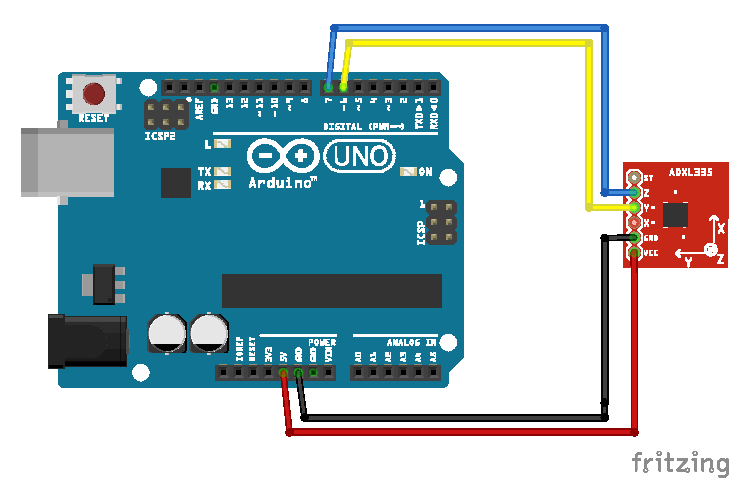
\includegraphics[width=\linewidth]{../6_Chapter6_UHF_R505/Picture/R505.pdf}
		\caption{R505 与 arduino的实物连接图}
		\label{fig:R505 与 arduino的实物连接图}
	\end{minipage}
	\hfill
	\begin{minipage}{.45\textwidth}
		\centering
		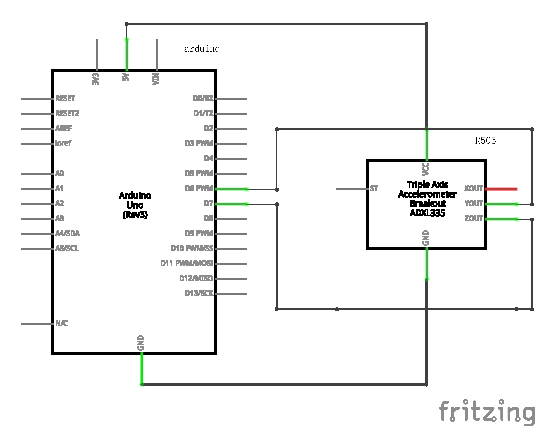
\includegraphics[width=\linewidth]{../6_Chapter6_UHF_R505/Picture/R505_line.pdf}
		\caption{R505 与 arduino的电路连接原理图}
		\label{fig:R505 与 arduino的电路连接原理图}
	\end{minipage}
\end{figure}

在程序中,本文使用了<SoftwareSerial.h>库,创建了软串口对象WIFISerial(6, 7),其中定义引脚6为RX,引脚7为TX(除了引脚0和引脚1以外的任意空闲数字引脚皆可,
其中引脚0和引脚1为Arduino默认的串口通讯接口,如果占用了可能会造成通讯堵塞) \\
\begin{itemize}
    \item 引脚6为RX 与 R505的TX连接;
    \item 引脚7为TX 与 R505的RX连接;
    \item 引脚5V 与 R505的VCC连接;
    \item 引脚GND 与 R505的GND连接;
    \item R505的使能引脚EN默认为高电平, 不需要连接。
\end{itemize}

UFID标签卡的存储空间分为四个区: RESERVED区, EPC区, TID区, USER区。其中EPC区作为识别标签对象的电子产品码, 用户可以手动输入修改。
由于我们使用的是"读多卡"的指令进行读, 所以返回的消息中第二位是'U', 与“读多卡”指令相对应。除了消息开头结尾固定的字符'0x0A'和'0x0D',还有
刚刚提到的'U',以外卡内还有32个字节, 其中前4个字节为商家编号例如“3000”,后四个字节为卡的ID编号,为每张卡所特有,
因此卡片的前四个字节和后四个字节最好不要对其进行修改。
中间24个字节可以随意存储,本文这里将这24个字节中前4个字节用于存储货物类型, 接着后面4个字节存储箱内单个物品的质量, 接着后面4个字节存储箱子外壳的质量。

当Arduino对R505进行控制, 需要通过创建的软串口“WIFISerial”使用“write”函数给R505发送不同指令, 待R505完成操作后可以通过软串口的“read”函数
一个字节一个字节的读取返回的信息。

\subsection{RC505类的声明}

\begin{lstlisting}
class RC505 {
private:
  SoftwareSerial WIFISerial = SoftwareSerial(6, 7);
public:
  char Type_Name[3];  
  long Single_Weight;
  long Shell_Weight;
  
  RC505();
  bool read(char *sub);
  void write();
};
\end{lstlisting}

默认构造函数: 其中软串口波特率38400是为了和RC505保持一致。
\begin{lstlisting}
RC505::RC505(){
  WIFISerial.begin(38400);
};	
\end{lstlisting}

在介绍读写函数之前, 首先介绍一下读写指令。不同的指令对应着不同地址的读写。
\begin{lstlisting}
  const unsigned char MultiEPC[] = {0x0A, 0x55, 0x2C, 0x52, 0x31, 0x2C, 0x31, 0x2C, 0x37, 0x0D}; //同时读取多张卡的指令
  const unsigned char WriteEPC[] = {0x0A, 0x57, 0x31, 0x2C,  //第一个0x31表示EPC区
                                    0x32, 0x2C,    //从第2个位置开始
                                    0x33, 0x2C,  //这里是写的三个字节, 最多八个地址,每个地址4字节
                                    0x30, 0x30, 0x3A, 0x3A, //物品种类
                                    0x30, 0x30, 0x31, 0x30, //单个物品质量
                                    0x30, 0x30, 0x30, 0x30, 0x0D};  //外壳质量  
\end{lstlisting}

getMessage返回的是完整的消息, 将读取到的消息更新在传入的字符数组sub中。
\begin{itemize}
  \item 第一步: 向RC505写入读的指令后, 判断当前读到的字符是不是LF, 来决定是否开始接收接下来的字符;
  \item 第二步: 接收字符, 直到接收长度达33为止;
  \item 第三步: 更新RC505类中的Type\_Name和Single\_Weight。
\end{itemize}

\begin{lstlisting}
bool RC505::read(char *sub){
  WIFISerial.write(MultiEPC, sizeof(MultiEPC));
  
  int start1 = 0;
  unsigned char buffer = 0;
  int i=0;
  
  while(WIFISerial.available() > 0) { 
    buffer = (char)WIFISerial.read();   //获取串口接收到的数据

    if(start1 == 0 && buffer == LF){  //当读取到第一个字节为LF
      start1 = 1;
      continue;
    }

    if(start1 == 1 && buffer != CR){  //结尾标志CR和LF
      // Serial.print((char)buffer);
      sub[i]=(char)buffer; 
      i++;
      if(i==arrayMax) {
        // Serial.println(' ');
        break;
      }   
      continue;
    }

  }

  int w=0;
  for (int i=7;i<9;i++) Type_Name[i-7]=sub[i];
  for (int i=11;i<13;i++) {
    w += (sub[i]-48)*pow(10,12-i);
    // Serial.println(w);
  }
  Single_Weight=w;
  return 1;
};
\end{lstlisting}

write通过向RC505写入指令, 来间接写卡:
\begin{lstlisting}
void RC505::write(){
  WIFISerial.write(WriteEPC, sizeof(WriteEPC));
};
\end{lstlisting}

\subsection{RC505.ino}
与上一章RC522.ino相比, 就是把RC522的内容换成了RC505的内容, 然后更新RC505中Type\_Name和Single\_Weight。由于本身RC505中读写的函数几乎没有
判断读写状态的条件语句, 所以反而这里主程序能实现重量发生变化时, 直接发送消息, 不必反复进出刷卡。
\begin{lstlisting}
#include "master.h"
#include "transform.h"
#include "Surface.h"
#include "Calibrate.h"
#include "Oled.h"
#include "RC522.h"
#include "RC505.h"

master m1;
Surface YL_Surface;
Calibrate YL_Calibrated;
transform tf;
Oled oled;
RC522 rc522;
RC505 rc505;

long numbefore=0, numnow=1;
char te[3];
unsigned long Sweight;
char MessageNow[arrayMax];
bool flag=0; //1--->write; 0--->read

void setup() {
  //设置串口波特率38400
  Serial.begin(38400);
  m1.initialize(8);    //8needschanged
  YL_Calibrated.setpin_SCKDT(4, 5);
  YL_Calibrated.set_range(20);
  YL_Calibrated.kb_Initialize();
  oled.initialize();  
  rc522.initialize(9,10);
}


void loop() { 
  switch(flag){
    case 0: 
      // while(1) {
      //   bool state = rc505.write();
      //   if(state==1)
      //     break;
      // }   
      rflag=1;
      // break;
    case 1:
      while(1) {
        bool state = rc505.read(MessageNow);
        if(state==1)
          break;
      }
      break;
  }  
  for (int i=0; i<sizeof(rc505.Type_Name);i++) te[i]=rc505.Type_Name[i];
  Sweight=rc505.Single_Weight;

  numbefore = numnow;
  unsigned long CalibratedWeight = YL_Calibrated.Output_CalibratedWeight(YL_Surface.Get_Surface());
  numnow = ceil(CalibratedWeight/Sweight);

  bool flag= (numbefore==numnow?0:1);
  if(flag){
  tf.initialize(te, m1.address, numnow, CalibratedWeight);
  tf.pack();
  digitalWrite(3,HIGH);
  m1.send(9, tf.Transmission_Information);
  Serial.println(tf.Transmission_Information);
  oled.showIIC(te, numnow);
  digitalWrite(3,LOW);
  }

  delay(3000); 
}
\end{lstlisting}

\section{第七章: 部署}
这一章主要介绍实际如何部署好一个货架。一个完整的货架包含: 一个触摸屏, 多个电子秤还有整个架子。软件上需要给所有电子秤烧录好代码, 触摸屏的UI界面设计好; 
硬件上要连好Arduino和压力传感器, 读卡器等元器件的连线, 以及整个货架的IIC通信线路。上述过程分为四步来完成:
\begin{itemize}
  \item 第一步: 秤的组装;
  \item 第二步: 上传程序;
  \item 第三步: 货架布线;
  \item 第四步: 触摸屏显示;
\end{itemize}

\subsection{秤的组装}
压力测量模块连接, 详见第一章:
\begin{figure}[h]
	\centering
	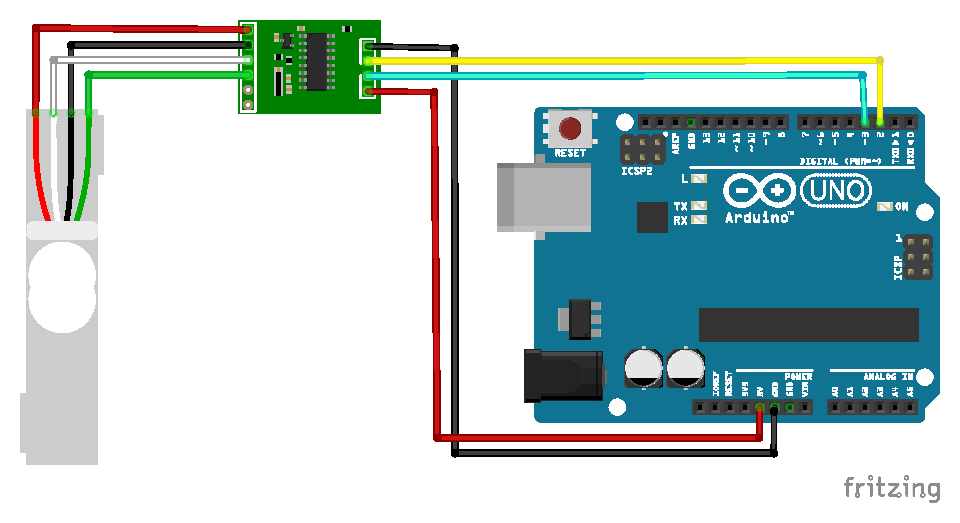
\includegraphics[width=\linewidth]{../1_Chapter1_RAW/Picture/PressureSensor.pdf}
	\caption{压力测量模块流程}
	\label{fig:压力测量模块流程图}
	\hfill
\end{figure}
		
两种读卡器连接, 详见第五章第六章:
\begin{figure}[h]
	\centering
	\begin{minipage}{.45\textwidth}
		\centering
		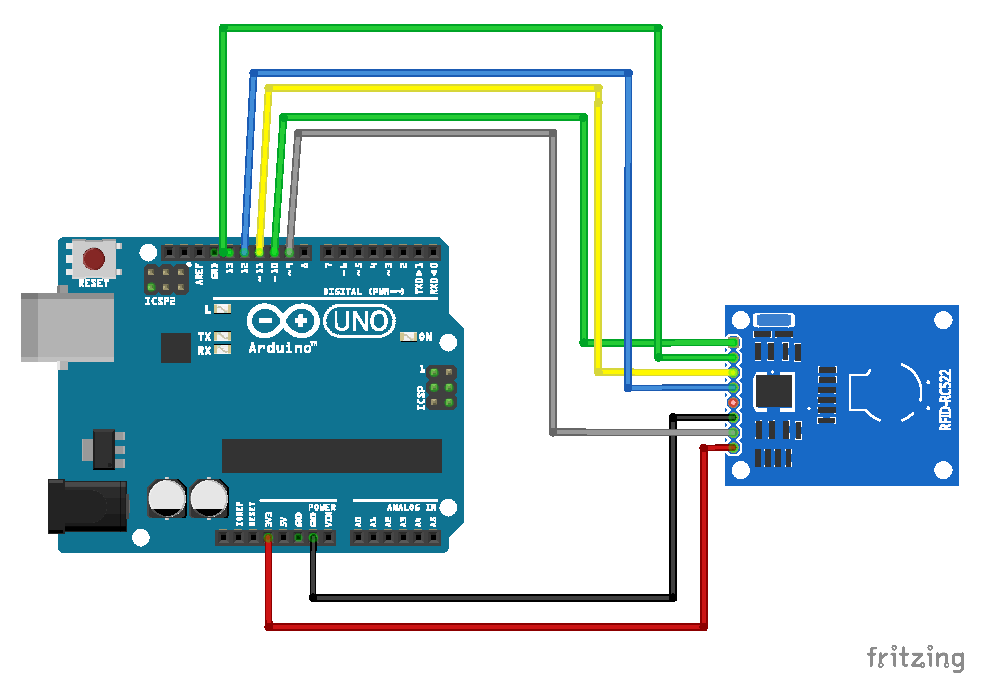
\includegraphics[width=\linewidth]{../5_Chapter5_RC522/Picture/RFID_RC522.pdf}
		\caption{RC522硬件连接}
		\label{fig:RC522硬件连接}
	\end{minipage}%
	\hfill
  \begin{minipage}{.45\textwidth}
		\centering
		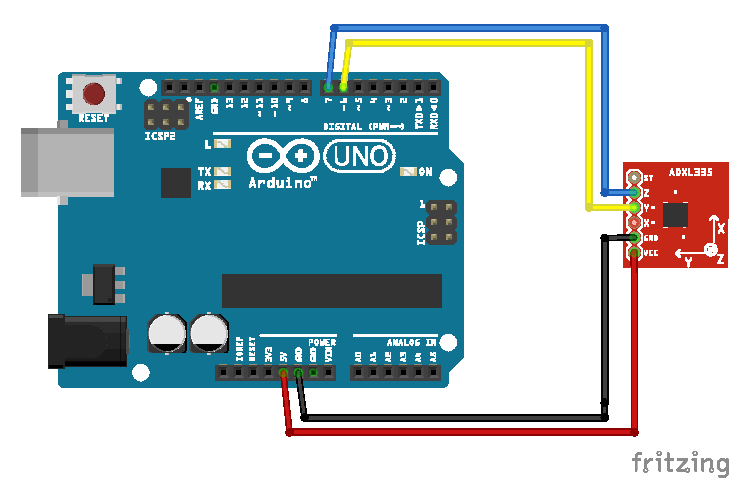
\includegraphics[width=\linewidth]{../6_Chapter6_UHF_R505/Picture/R505.pdf}
		\caption{R505 与 arduino的实物连接图}
		\label{fig:R505 与 arduino的实物连接图}
	\end{minipage}
\end{figure}

\subsection{上传程序}
这里我们选择的是TCA9548A的布线方式, arduino分为多个主机一个从机, 

\noindent 主机:
如果是采取近的读卡器读取物品种类及单个物体质量信息, 就烧录下面的程序:
\begin{lstlisting}
  #include "master.h"
  #include "transform.h"
  #include "Surface.h"
  #include "Calibrate.h"
  #include "Oled.h"
  #include "RC522.h"
  
  master m1;
  Surface YL_Surface;
  Calibrate YL_Calibrated;
  transform tf;
  Oled oled;
  RC522 rc522;
  
  long numbefore=0, numnow=1;
  char te[3];
  unsigned long Sweight;
  bool rflag=1;  //1 ---> read; 0 ---> write
  
  void setup() {
    Serial.begin(9600);
    m1.initialize(8);    //8needschanged
    YL_Calibrated.setpin_SCKDT(4, 5);
    YL_Calibrated.set_range(20);
    YL_Calibrated.kb_Initialize();
    oled.initialize();  
    rc522.initialize(9,10);
  }
  
  void loop() {
    switch(rflag){
      case 0: 
        while(1) {
          bool state = rc522.write();
          if(state==1)
            break;
        }   
        rflag=1;
        break;
      case 1:
        while(1) {
          bool state = rc522.read();
          if(state==1)
            break;
        }
        break;
    }
    for (int i=0; i<sizeof(rc522.Type_Name);i++) te[i]=rc522.Type_Name[i];
    Sweight=rc522.Single_Weight;
  
    numbefore = numnow;
    unsigned long CalibratedWeight = YL_Calibrated.Output_CalibratedWeight(YL_Surface.Get_Surface());
    numnow = ceil(CalibratedWeight/Sweight);
  
    bool flag= (numbefore==numnow?0:1);
    if(flag){
    tf.initialize(te, m1.address, numnow, CalibratedWeight);
    tf.pack();
    digitalWrite(3,HIGH);
    m1.send(9, tf.Transmission_Information);
    Serial.println(tf.Transmission_Information);
    oled.showIIC(te, numnow);
    digitalWrite(3,LOW);
    }
  
    delay(3000);
  }  
\end{lstlisting}

如果是采取远的读卡器读取物品种类及单个物体质量信息, 就烧录下面的程序:
\begin{lstlisting}
  #include "master.h"
  #include "transform.h"
  #include "Surface.h"
  #include "Calibrate.h"
  #include "Oled.h"
  #include "RC522.h"
  #include "RC505.h"
  
  master m1;
  Surface YL_Surface;
  Calibrate YL_Calibrated;
  transform tf;
  Oled oled;
  RC522 rc522;
  RC505 rc505;
  
  long numbefore=0, numnow=1;
  char te[3];
  unsigned long Sweight;
  char MessageNow[arrayMax];
  bool flag=0; //1--->write; 0--->read
  
  void setup() {
    //设置串口波特率38400
    Serial.begin(38400);
    m1.initialize(8);    //8needschanged
    YL_Calibrated.setpin_SCKDT(4, 5);
    YL_Calibrated.set_range(20);
    YL_Calibrated.kb_Initialize();
    oled.initialize();  
    rc522.initialize(9,10);
  }
  
  
  void loop() { 
    switch(flag){
      case 0: 
        // while(1) {
        //   bool state = rc505.write();
        //   if(state==1)
        //     break;
        // }   
        rflag=1;
        // break;
      case 1:
        while(1) {
          bool state = rc505.read(MessageNow);
          if(state==1)
            break;
        }
        break;
    }  
    for (int i=0; i<sizeof(rc505.Type_Name);i++) te[i]=rc505.Type_Name[i];
    Sweight=rc505.Single_Weight;
  
    numbefore = numnow;
    unsigned long CalibratedWeight = YL_Calibrated.Output_CalibratedWeight(YL_Surface.Get_Surface());
    numnow = ceil(CalibratedWeight/Sweight);
  
    bool flag= (numbefore==numnow?0:1);
    if(flag){
    tf.initialize(te, m1.address, numnow, CalibratedWeight);
    tf.pack();
    digitalWrite(3,HIGH);
    m1.send(9, tf.Transmission_Information);
    Serial.println(tf.Transmission_Information);
    oled.showIIC(te, numnow);
    digitalWrite(3,LOW);
    }
  
    delay(3000); 
  }
\end{lstlisting}

\noindent 从机(也就是与TCA9548A相连的arduino板上的主程序如下):
\begin{lstlisting}
#include "Oled.h"
#include "slave.h"
#include "transform.h"

String slave::comdata="";

Oled oled;
slave s;
transform tf;

void setup() {
  Serial.begin(9600);
  s.initialize(8);
  oled.initialize();
  pinMode(7,INPUT);
  digitalWrite(7, LOW);
}

void loop() {
  tf.unpack(s.comdata);
  oled.showIIC(tf.Type_Name, tf.Number, tf.DEVICE_ADDRESS);
  delay(1000);
}
\end{lstlisting}

\newpage
\subsection{货架布线}
IIC通信及OLED屏显示连线, 详见第三章第四章:
\begin{figure}[h]
  \centering
  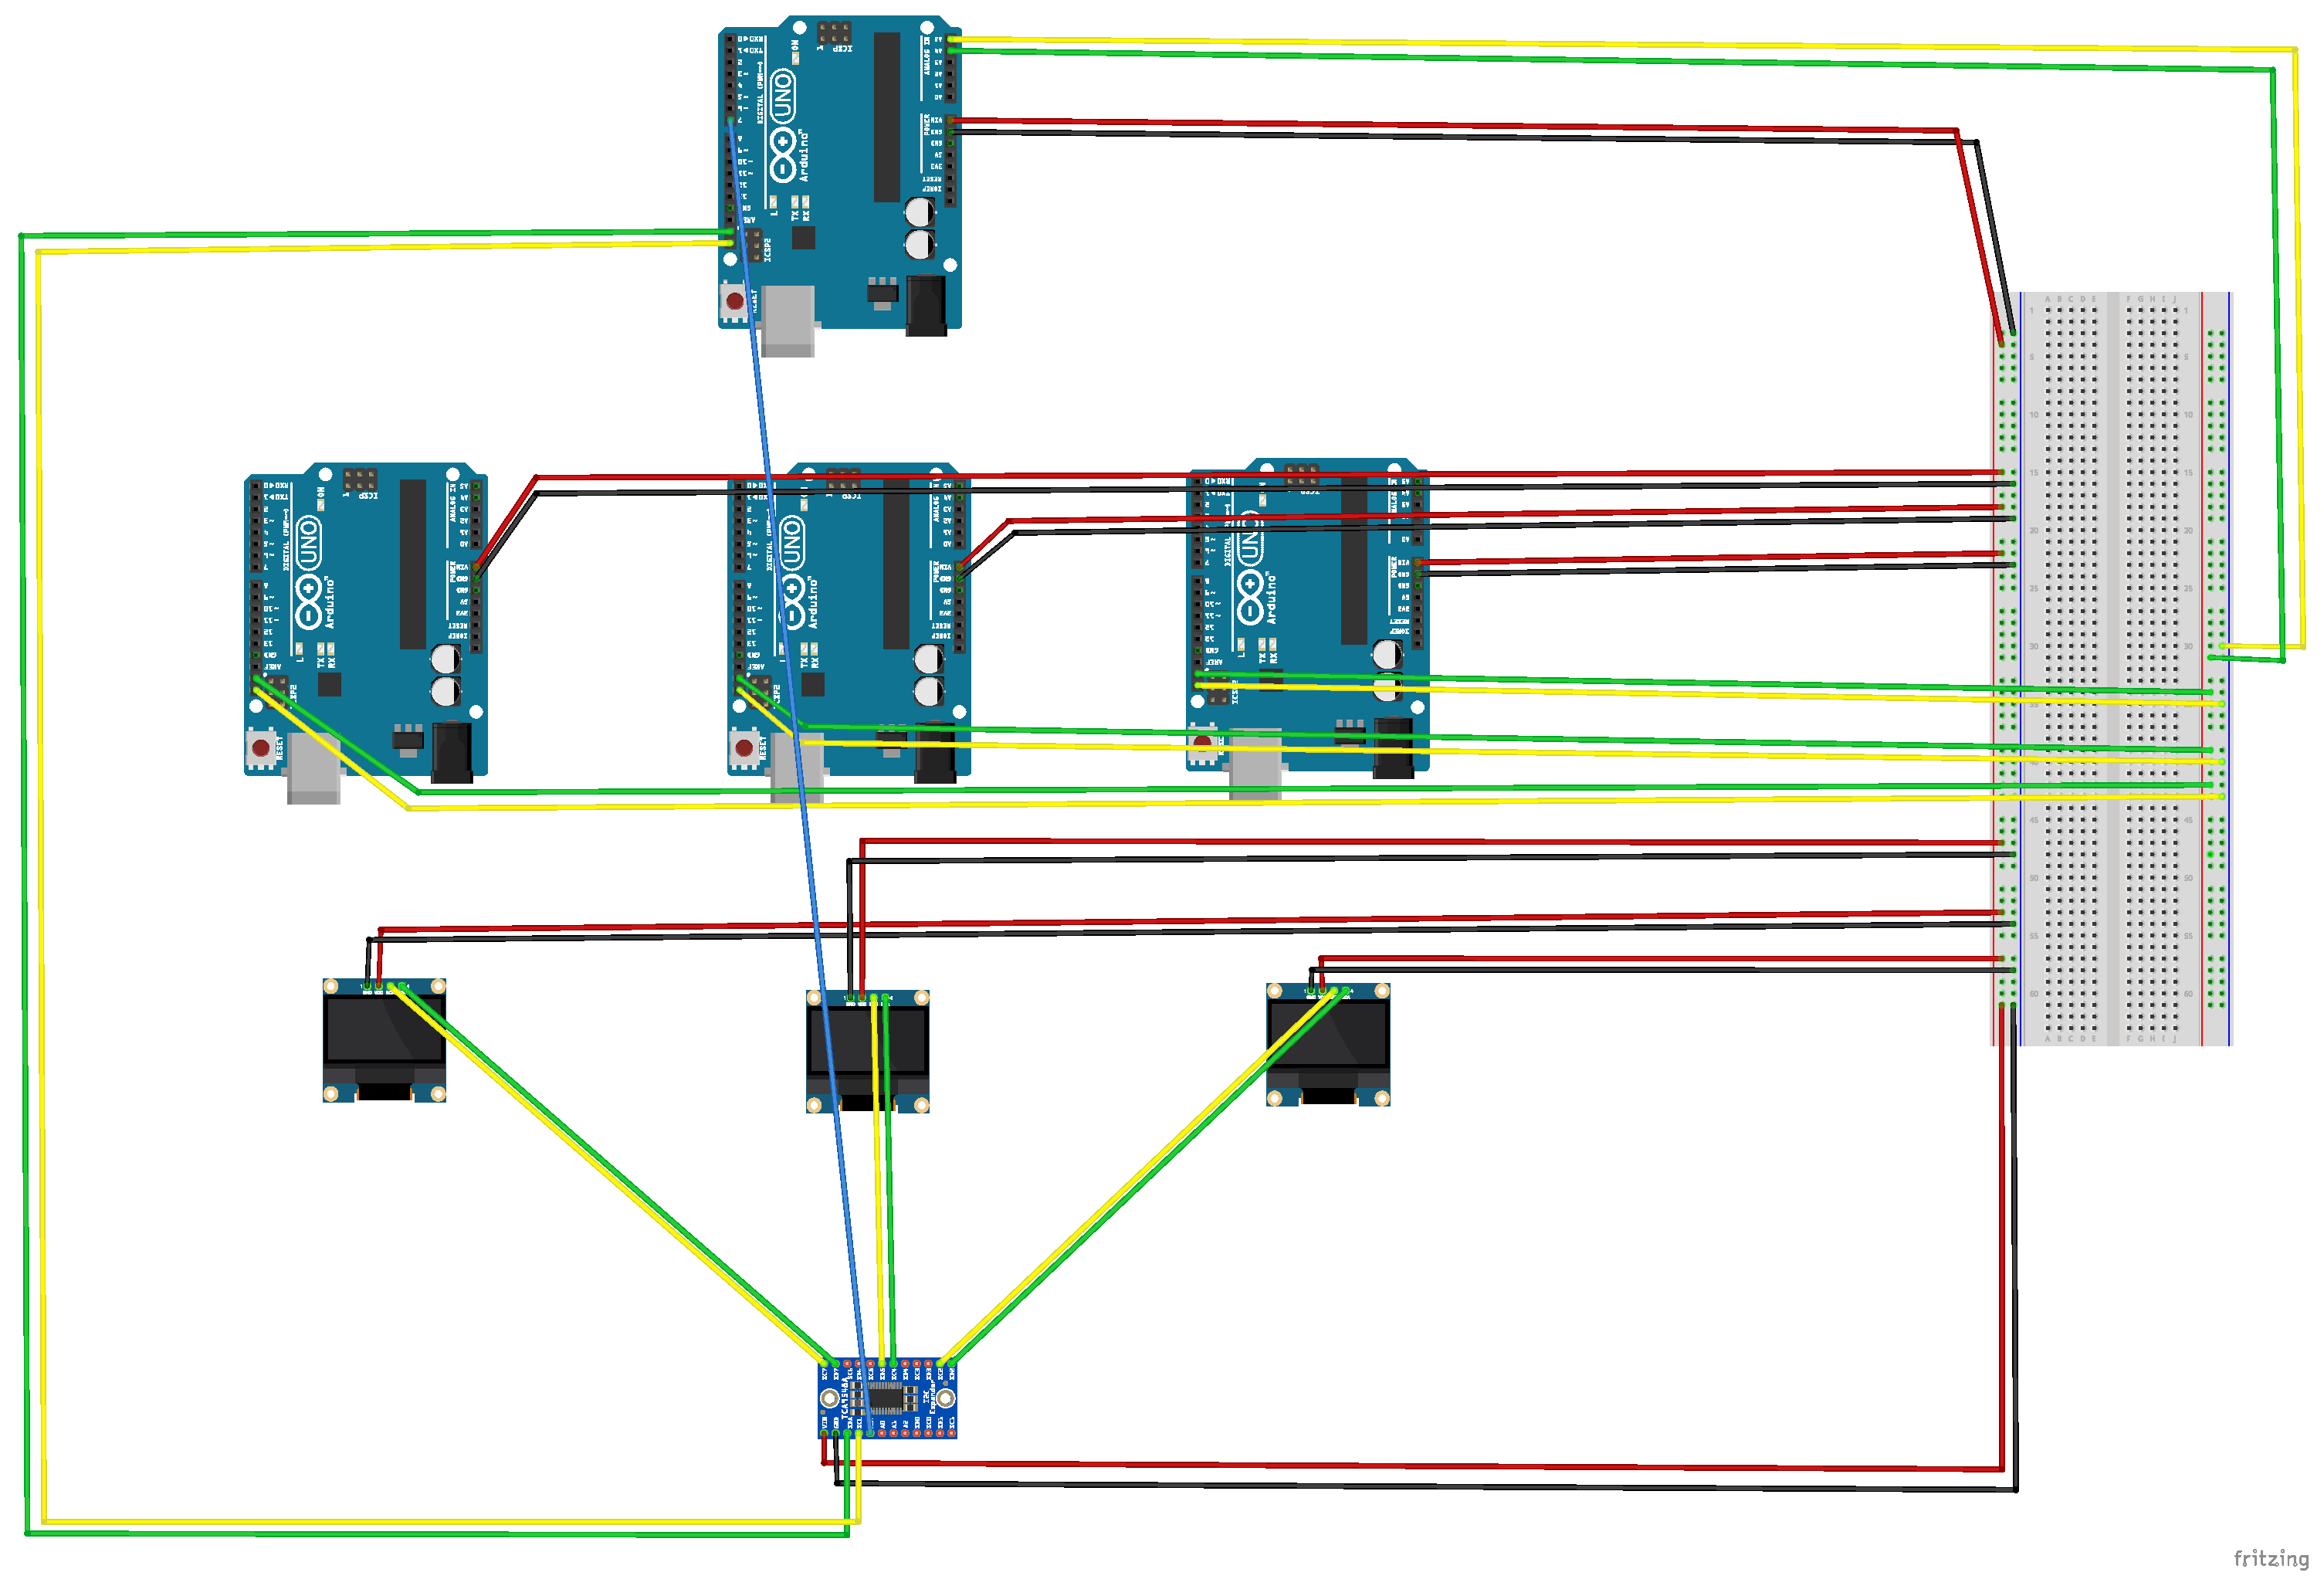
\includegraphics[width=0.8\textwidth]{../4_Chapter4_COMMUNICATION/Picture/一层货架示意图.pdf}
  \caption{一层货架示意图}
  \label{fig:一层货架示意图}
\end{figure}

对于第二层甚至更多层的话, 就要考虑总的电子秤数量是否超过8, 超过了的话则需要更多从机和TCA9548A模块。

\subsection{触摸屏显示}
上传下面的python代码到树莓派上运行, 树莓派就可以接收到从机发来的信号, 从而在屏幕上显示对应电子秤的重量变化。

\begin{lstlisting}
import sys
from PyQt5.QtWidgets import QApplication, QWidget, QVBoxLayout, QHBoxLayout, QGridLayout, QLabel, QMainWindow
from PyQt5.QtGui import QPixmap
from PyQt5.QtCore import Qt, QTimer, QIODevice, QByteArray
from PyQt5.QtSerialPort import QSerialPort, QSerialPortInfo
from qt_material import apply_stylesheet
from PyQt5.uic import loadUi


class MainWindow(QMainWindow):
    def __init__(self):
        super().__init__()
        loadUi("main_window1.ui", self)  # 加载UI文件
        # 设置窗口标题和大小
        self.setWindowTitle('货物管理')

        # 创建网格布局
        grid = QGridLayout(self)
        grid.setAlignment(Qt.AlignCenter)

        pixmap = QPixmap('jimu1.jpg')
        pixmap = pixmap.scaled(150, 130, Qt.KeepAspectRatio)
        self.label1.setPixmap(pixmap)
        self.label1.setFixedSize(pixmap.width(), pixmap.height())
        self.label1.setAlignment(Qt.AlignCenter)
        self.pushButton.clicked.connect(self.click_button)
        self.pushButton_2.clicked.connect(self.click_button2)

        # 应用Qt Material主题
        apply_stylesheet(self, theme='light_teal.xml')

        # 创建串口监视器
        self.serial = QSerialPort()
        self.serial.setPortName("COM3")  # 设置端口号
        self.serial.setBaudRate(QSerialPort.Baud9600)
        self.serial.readyRead.connect(self.handle_serial_data)
        self.serial.open(QIODevice.ReadWrite)

    def click_button(self):
        self.serial.close()

    def click_button2(self):
        self.serial = QSerialPort()
        self.serial.setPortName("COM8")  # 设置端口号
        self.serial.setBaudRate(QSerialPort.Baud9600)
        self.serial.readyRead.connect(self.handle_serial_data)
        self.serial.open(QIODevice.ReadWrite)

    def handle_serial_data(self):
        # 读取串口数据
        data = self.serial.readAll().data()
        data_str = str(data, encoding='utf-8')
        print(data)
        # 处理数据
        module_data = data_str.split(',')
        for i, module_str in enumerate(module_data):
            # 如果模块数据不为空,则更新数量和种类
            if module_str:
                try:
                    type_, num = module_str.split(':')
                    self.update_module_info(i, type_, num)
                except ValueError as e:
                    print(f"Error: {e}. Received data: {module_str}")

    def update_module_info(self, module_num, type_, num):
        # 获取模块信息字典
        module_info = {
            0: {'num': None, 'type': 'AA', 'image': 'jimu1.jpg'},
            1: {'num': None, 'type': 'B', 'image': 'picture2.jpg'},
            2: {'num': None, 'type': 'C', 'image': 'picture3.jpg'},
            3: {'num': None, 'type': 'D', 'image': 'picture4.jpg'},
            4: {'num': None, 'type': 'E', 'image': 'picture5.jpg'},
            5: {'num': None, 'type': 'F', 'image': 'picture6.jpg'},
            6: {'num': None, 'type': 'G', 'image': 'picture7.jpg'},
            7: {'num': None, 'type': 'H', 'image': 'picture8.jpg'},
            8: {'num': None, 'type': 'I', 'image': 'picture9.jpg'},
            9: {'num': None, 'type': 'J', 'image': 'picture10.jpg'},
            10: {'num': None, 'type': 'K', 'image': 'picture11.jpg'},
            11: {'num': None, 'type': 'L', 'image': 'picture12.jpg'}
        }

        # 更新模块信息字典中对应模块的数量和种类
        for i in range(12):
            if module_info[i]['type'] == type_:
                module_info[i]['num'] = num
                num_label = self.findChild(QLabel, f'label_num_{i}')
                type_label = self.findChild(QLabel, f'label_type_{i}')
                if num_label is None:
                    print(f"label_num_{module_num} not found!")
                    return

                num_label.setText(num)
                break


if __name__ == '__main__':
    app = QApplication(sys.argv)
    main_window = MainWindow()
    main_window.show()
    sys.exit(app.exec_())  
\end{lstlisting}

\end{document} 

